% !TEX encoding = UTF-8 Unicode
\documentclass[12pt, A4,onecolumn]{article} %se puede poner twocolumn
\usepackage[normalem]{ulem} %tachar
\usepackage{cite}
\usepackage[utf8]{inputenc}
\usepackage{verbatim} %para comentarios 
%\usepackage[spanish]{babel}
\usepackage[hidelinks]{hyperref} %para que no salga en rojo
\usepackage{color} %para poder escribir con colores
\usepackage[margin=2.5cm]{geometry} %para modificar margenes
\usepackage{listings} %para insertar código
\usepackage[table,xcdraw]{xcolor} %para insertar tablas con color
\usepackage{amsmath} %para matrices
\usepackage{graphicx} %para insertar imagenes
\usepackage{float}
\usepackage{subcaption} % loads the caption package
\usepackage{multirow}
\definecolor{dkgreen}{rgb}{0,0.6,0}
\definecolor{gray}{rgb}{0.5,0.5,0.5}
\definecolor{mauve}{rgb}{0.58,0,0.82}
\graphicspath{ {Machintosh_HD/Utenti/admin/Scrivania} }


\title{\textbf{Machine Learning\\ 
\small{by Stanford University}\\
Week\_4
}}
\author{
Jose Vicente Yago Martínez
}%\date{28/3/2019}


\begin{document}
\maketitle

	
%\vfill
%\centering
%\textit{Lecturer:} \\
%AndrewNg


%\begin{figure}[H]
%	\centering
%	\includegraphics[width=0.2\textwidth]{logo-fium}
%\end{figure}	



\newpage
\tableofcontents
%\listoffigures

\newpage

% -----------------------------------------------------------------------------------%
% -----------------------------------------------------------------------------------%
%------------------------------------INTRO---------------------------------------%
% -----------------------------------------------------------------------------------%
% -----------------------------------------------------------------------------------%

\section{Neural networks}
\subsection{Model representation I}

\begin{figure}[H]
	\centering
	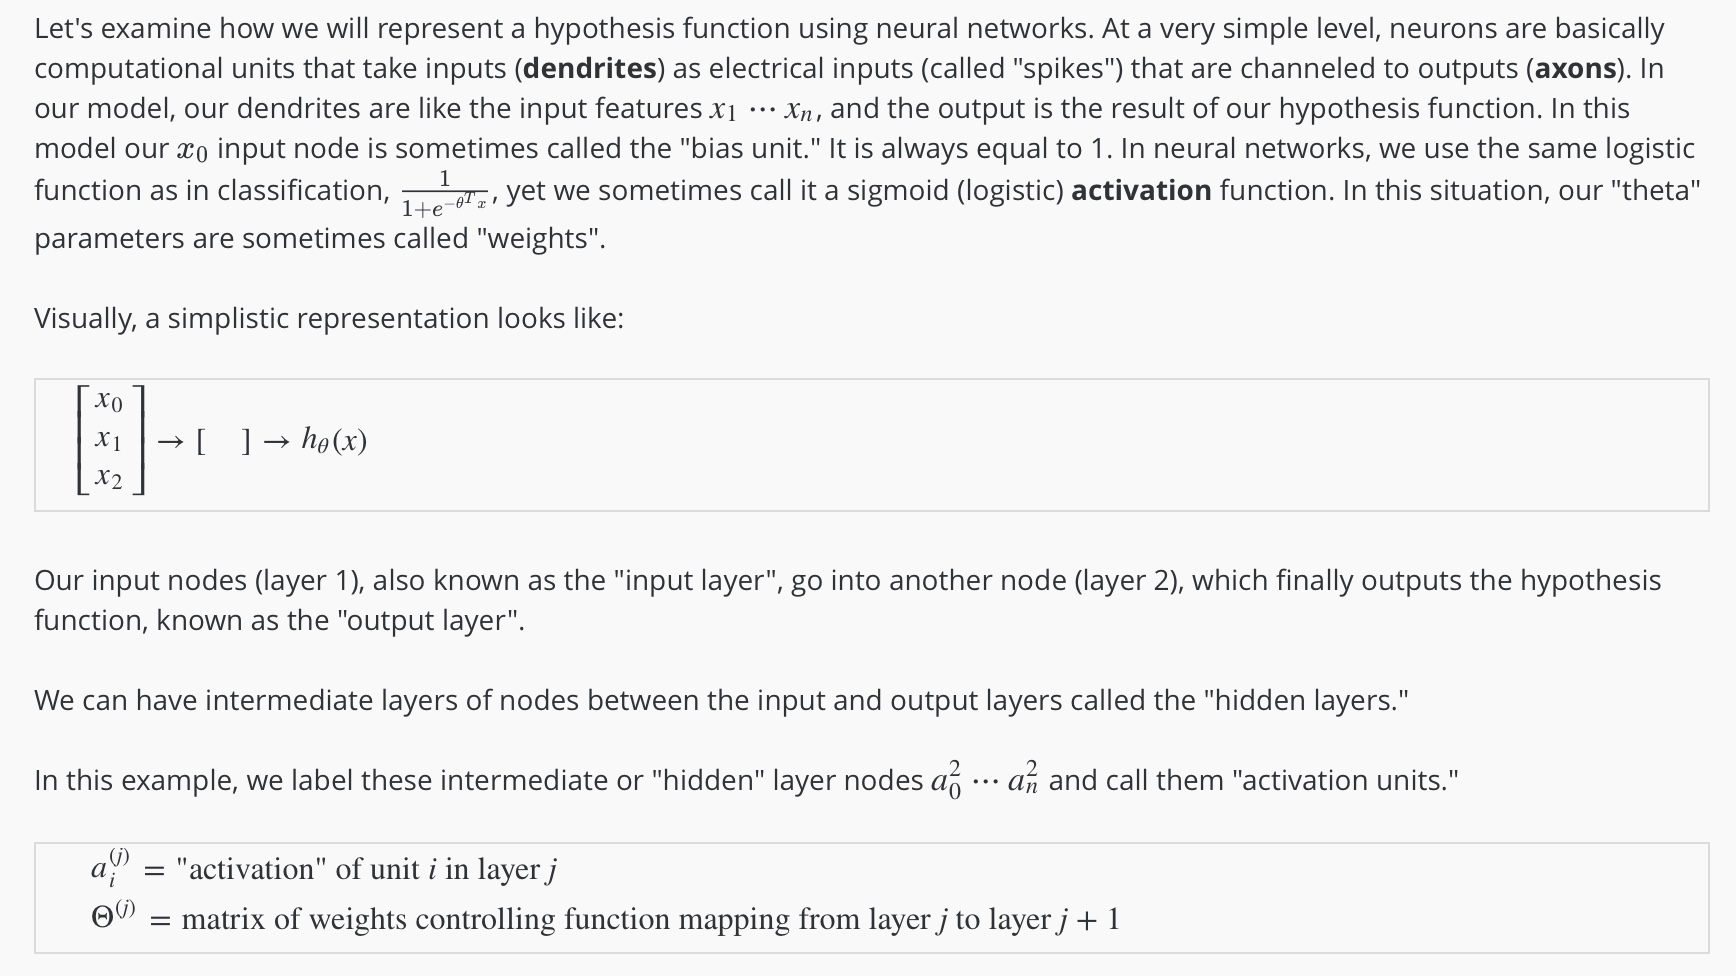
\includegraphics[width=1\textwidth]{./ImagenesW4/modelRep1}
\end{figure}

\begin{figure}[H]
	\centering
	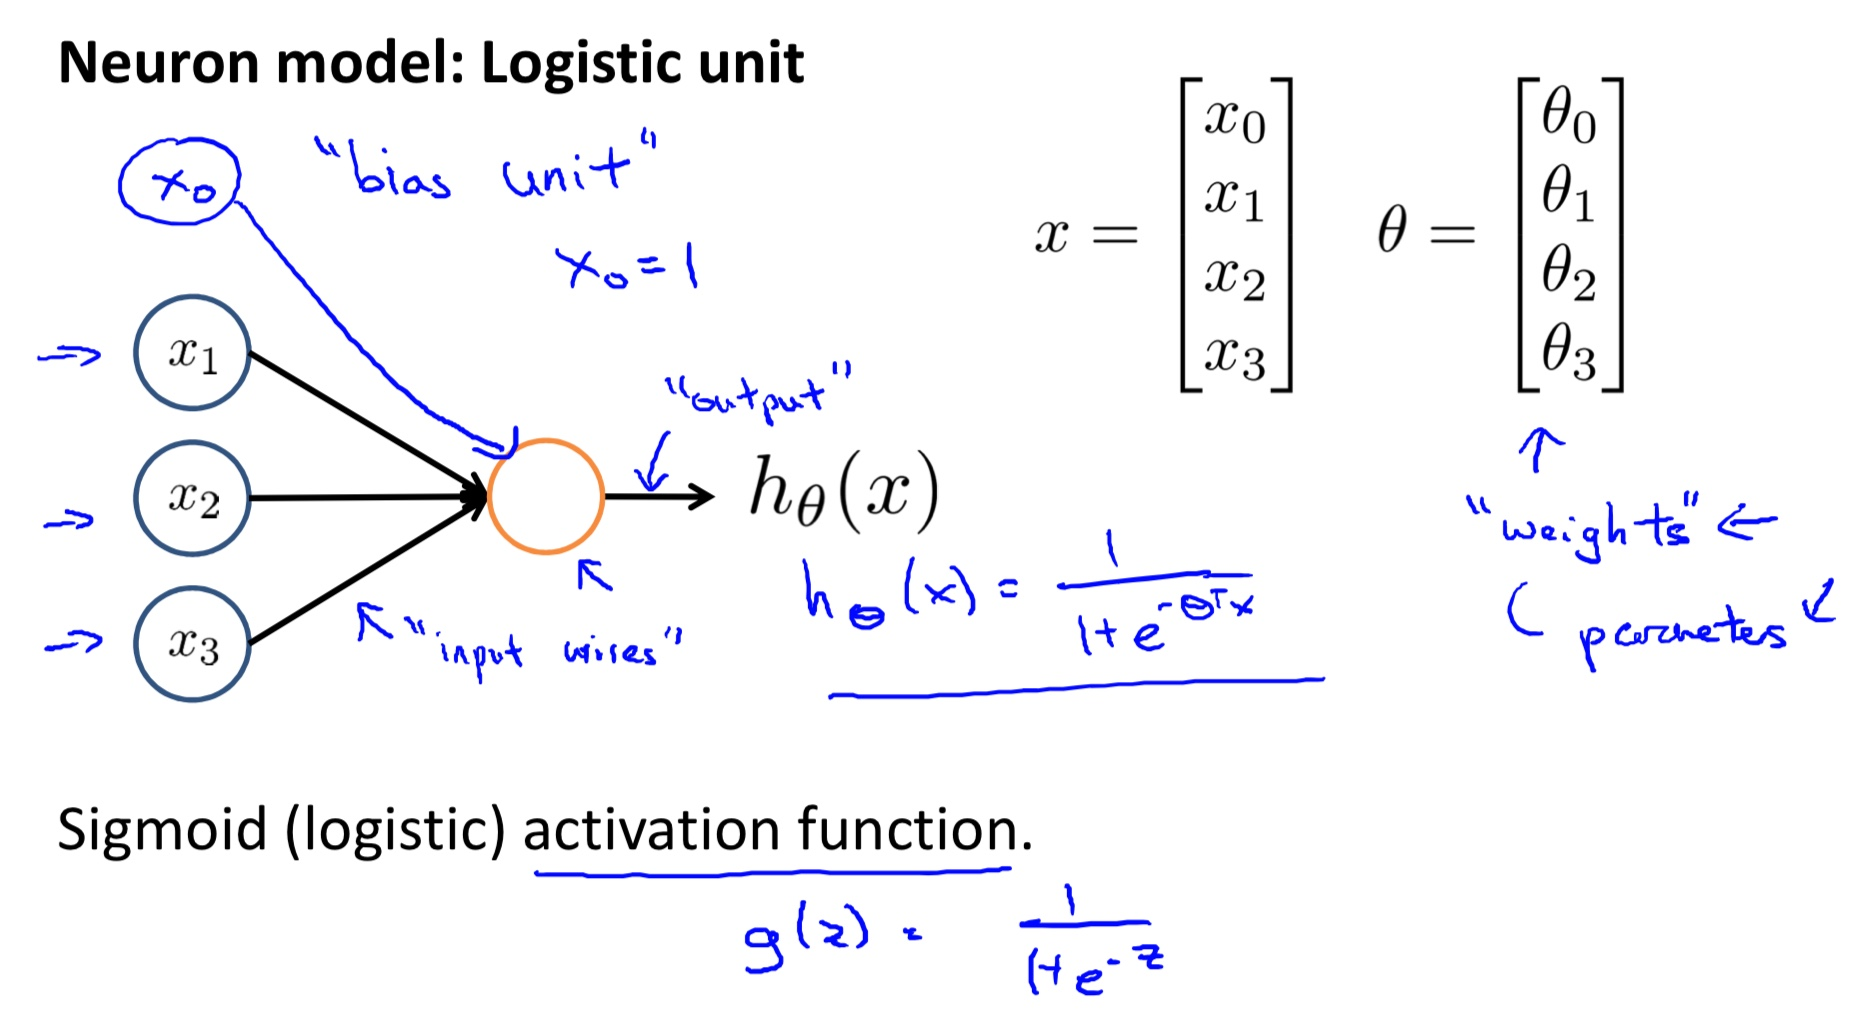
\includegraphics[width=1\textwidth]{./ImagenesW4/neuroModel1}
\end{figure}

\begin{figure}[H]
	\centering
	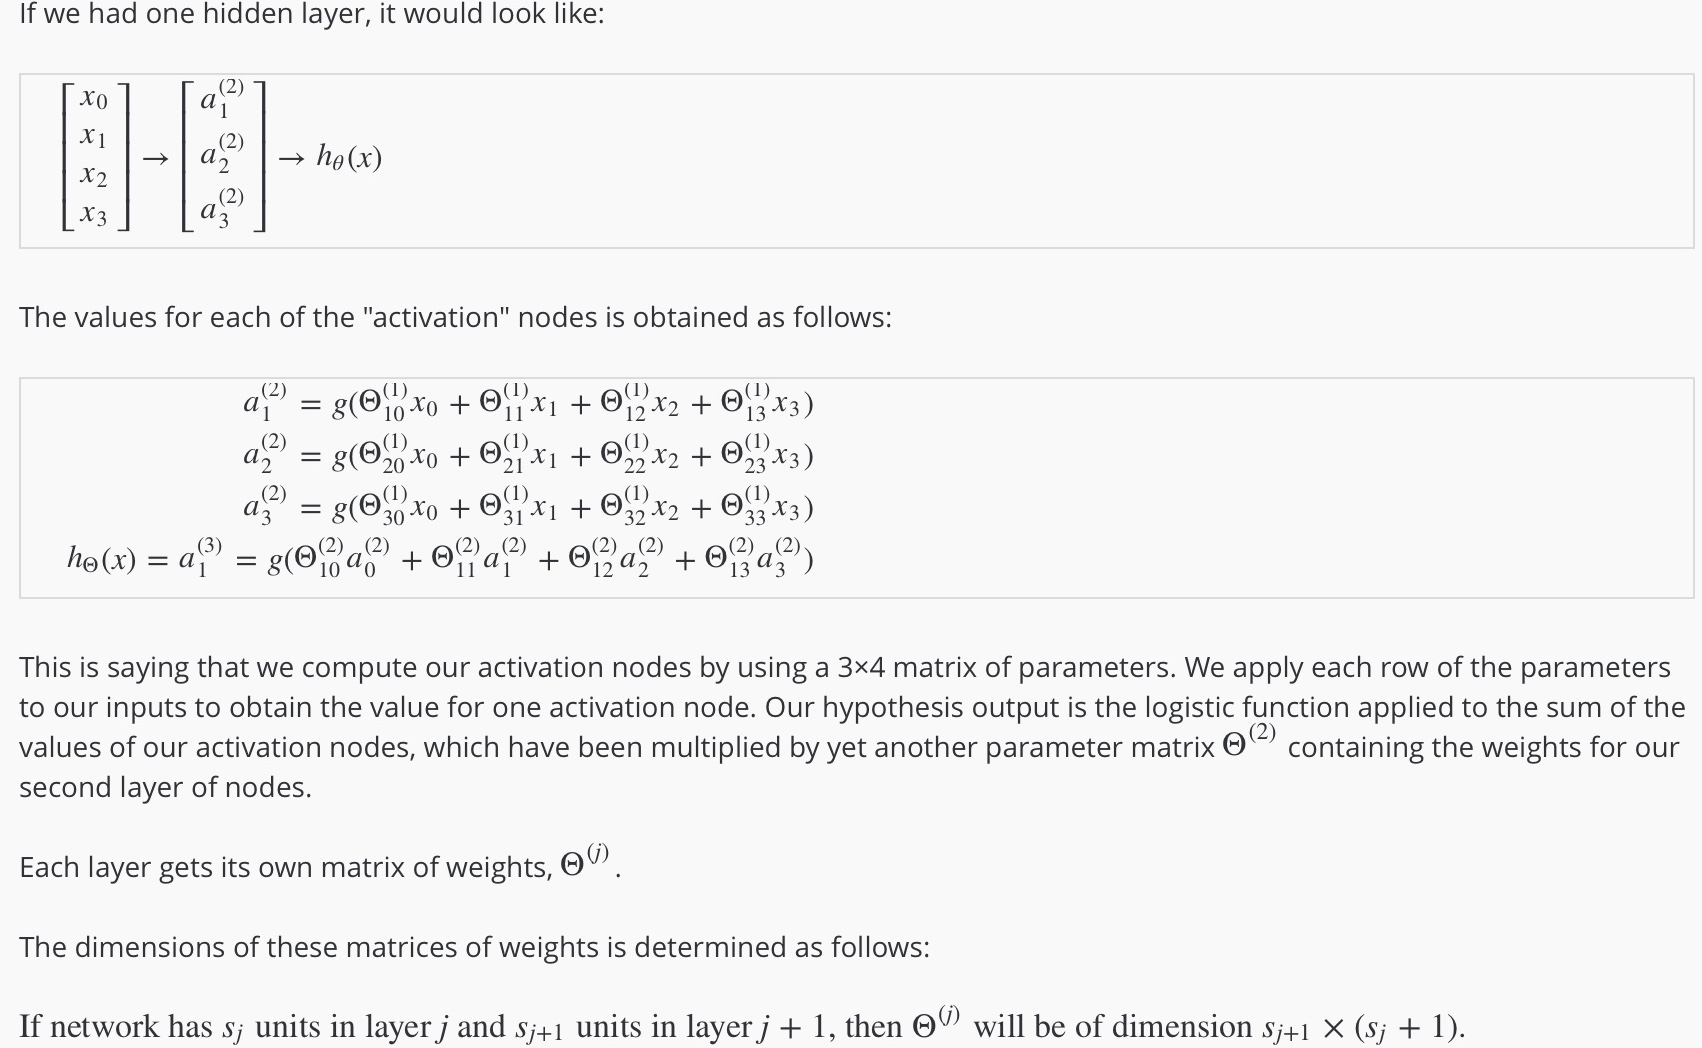
\includegraphics[width=1\textwidth]{./ImagenesW4/modelRep2}
\end{figure}

\begin{figure}[H]
	\centering
	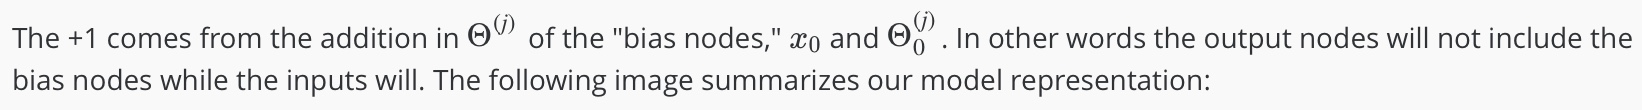
\includegraphics[width=1\textwidth]{./ImagenesW4/modelRep3}
\end{figure}

\begin{figure}[H]
\minipage{0.5\textwidth}
  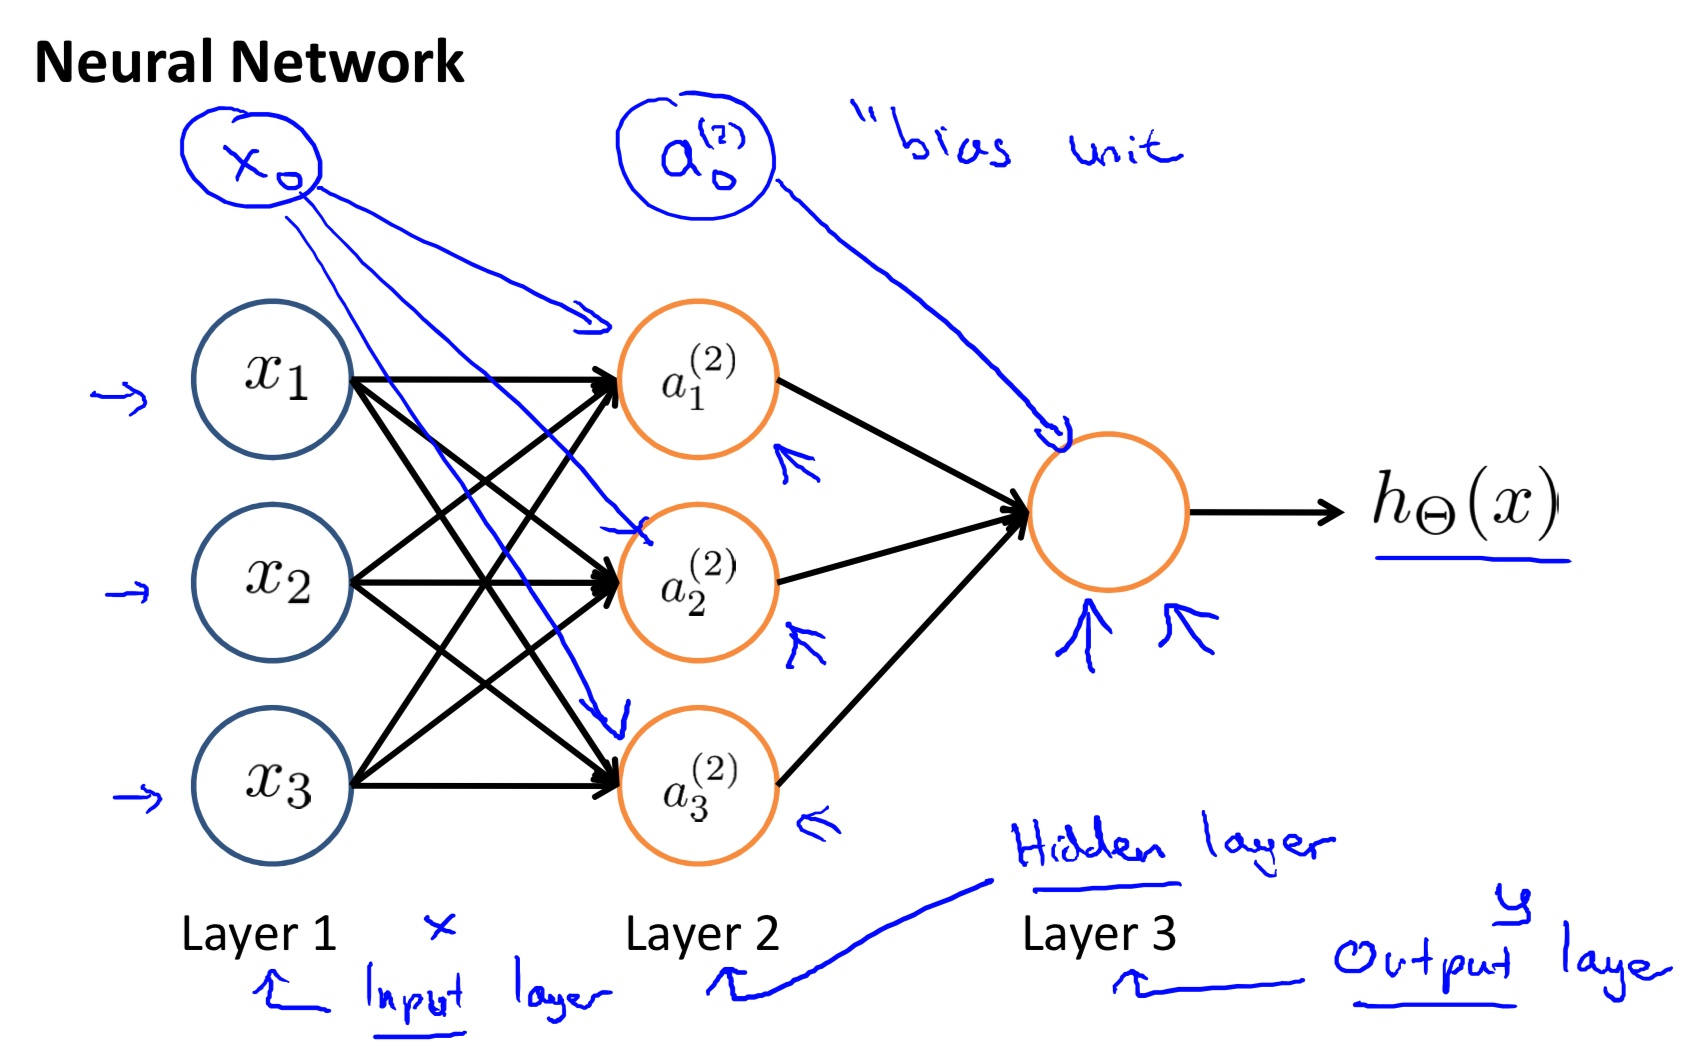
\includegraphics[width=\linewidth]{./ImagenesW4/neuralNetwork1}
\endminipage\hfill
\minipage{0.525\textwidth}
  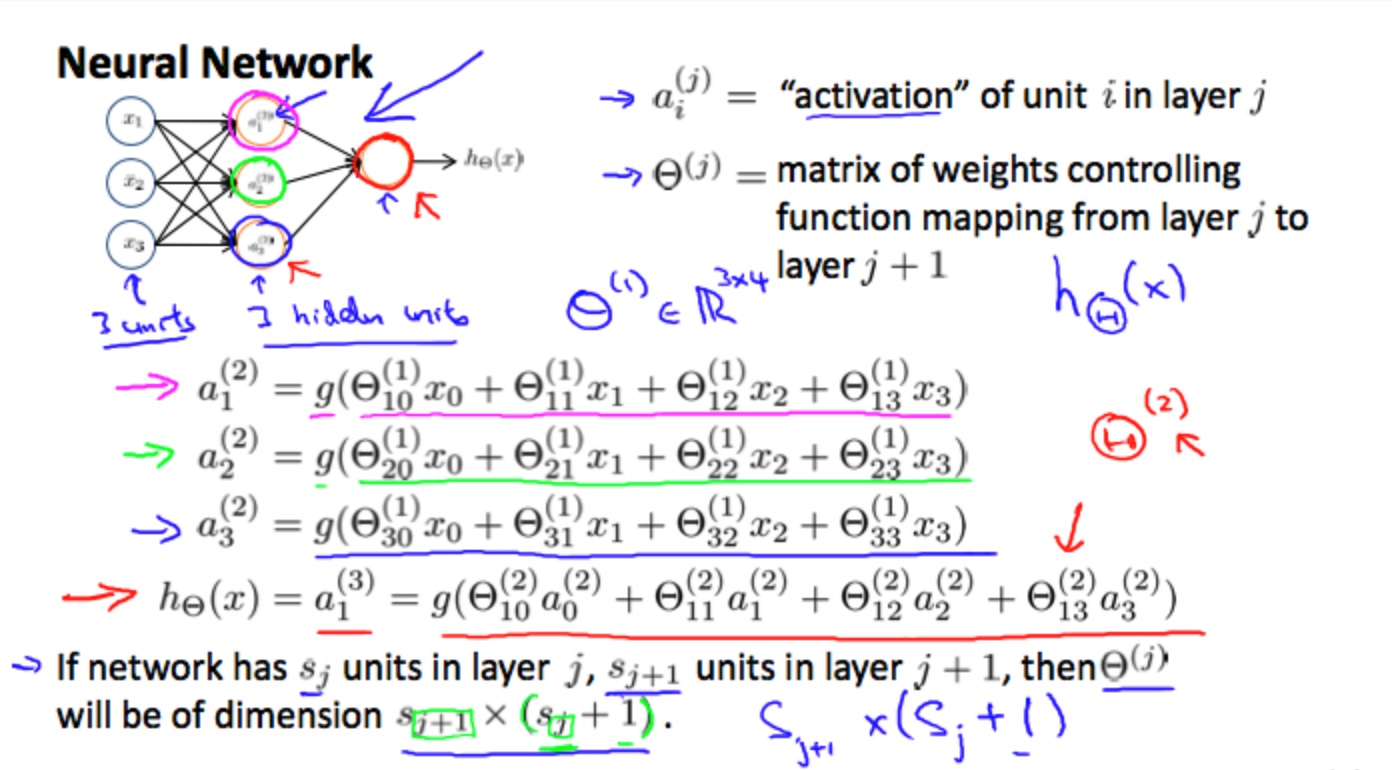
\includegraphics[width=\linewidth]{./ImagenesW4/modelRep4}
\endminipage\hfill
\end{figure}

\begin{figure}[H]
	\centering
	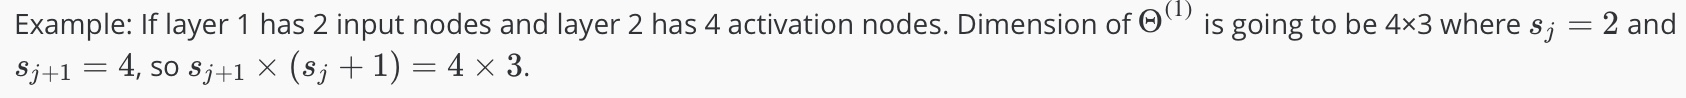
\includegraphics[width=1\textwidth]{./ImagenesW4/modelRep5}
\end{figure}

\begin{figure}[H]
	\centering
	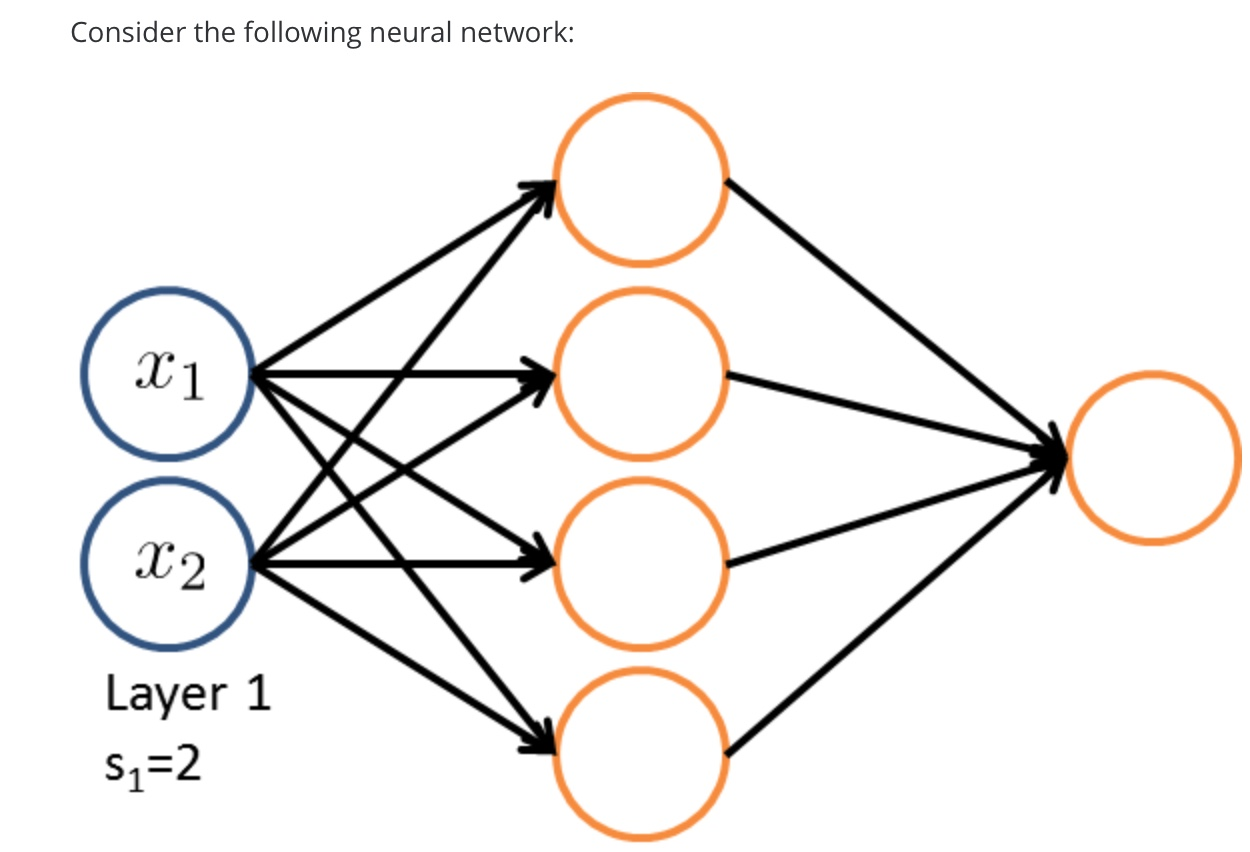
\includegraphics[width=1\textwidth]{./ImagenesW4/testmrep1_1}
\end{figure}

\begin{figure}[H]
	\centering
	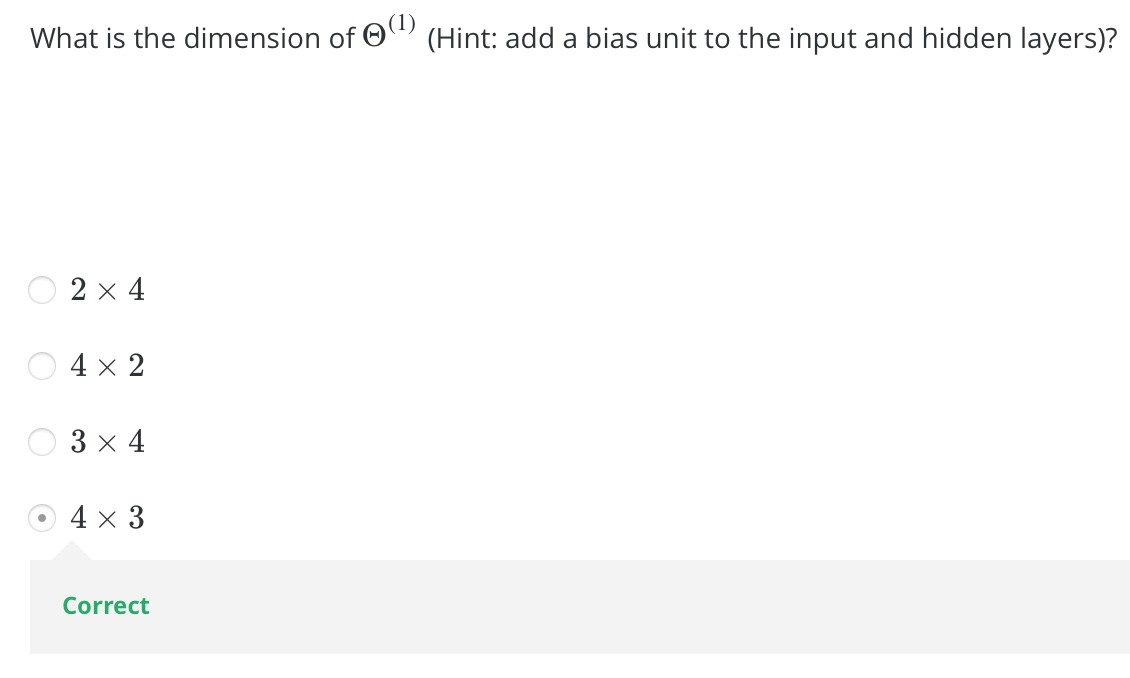
\includegraphics[width=1\textwidth]{./ImagenesW4/testmrep1_2}
\end{figure}


\subsection{Model representation II}
\begin{figure}[H]
	\centering
	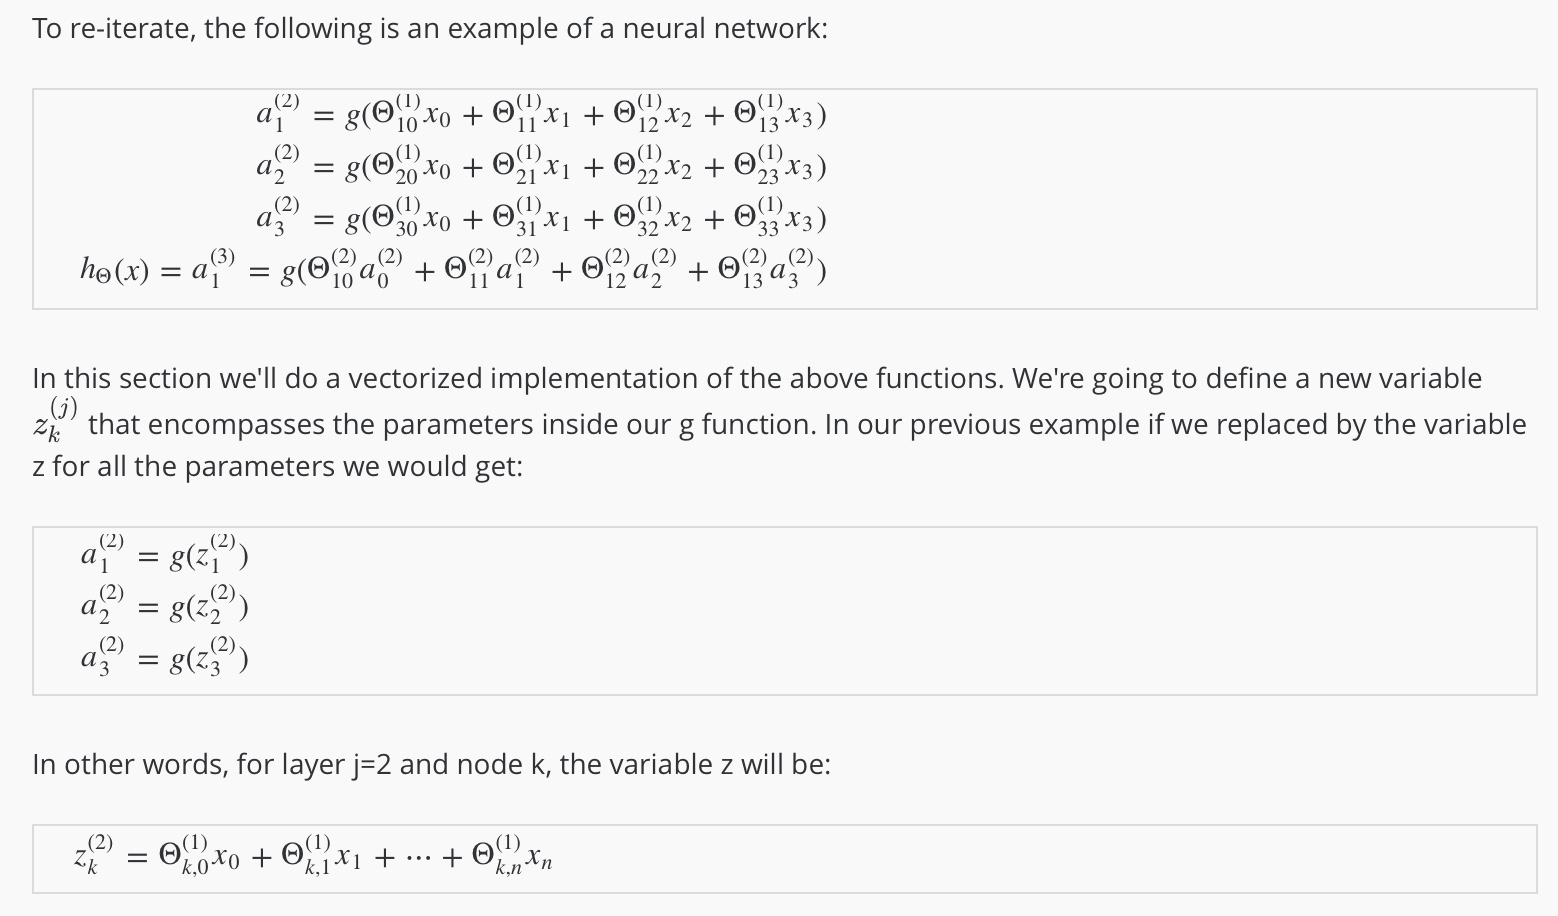
\includegraphics[width=1\textwidth]{./ImagenesW4/modelRep6}
\end{figure}

\begin{figure}[H]
	\centering
	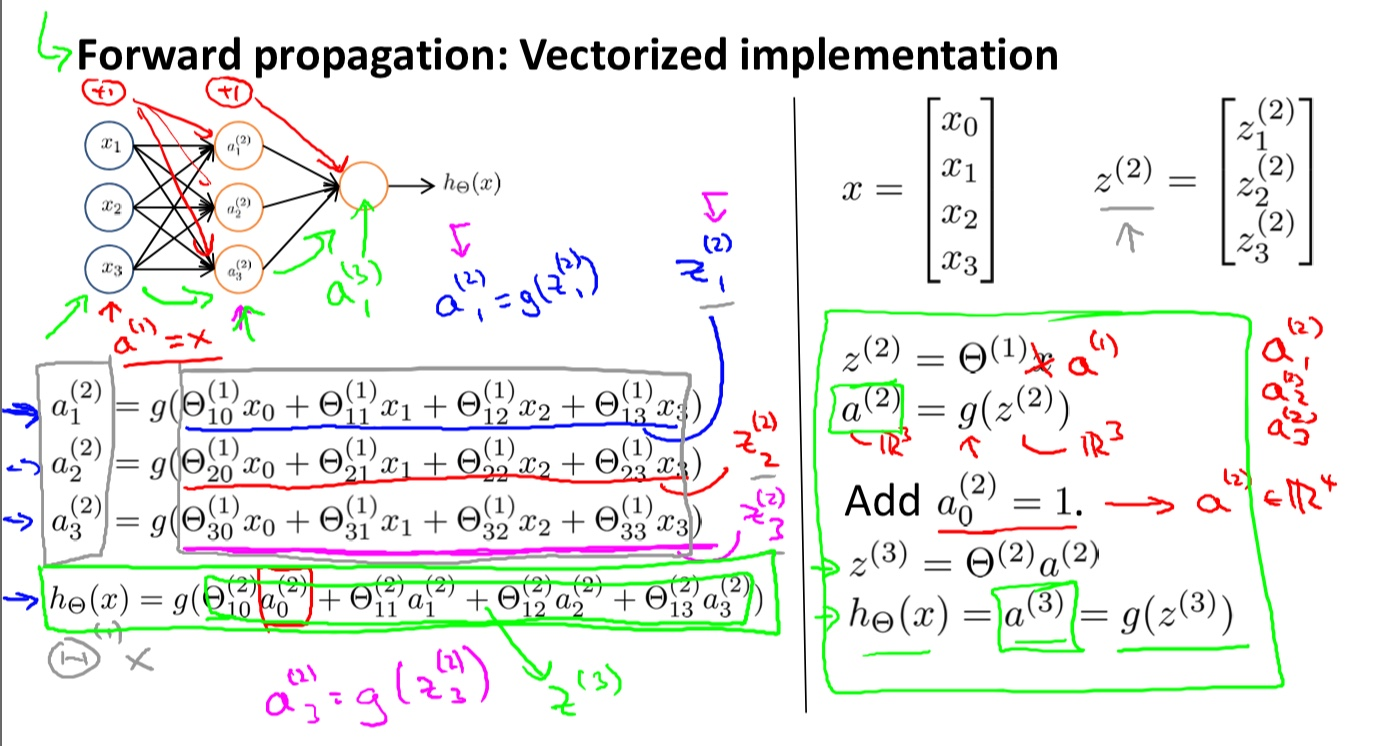
\includegraphics[width=1\textwidth]{./ImagenesW4/forwardProp1}
\end{figure}

\begin{figure}[H]
	\centering
	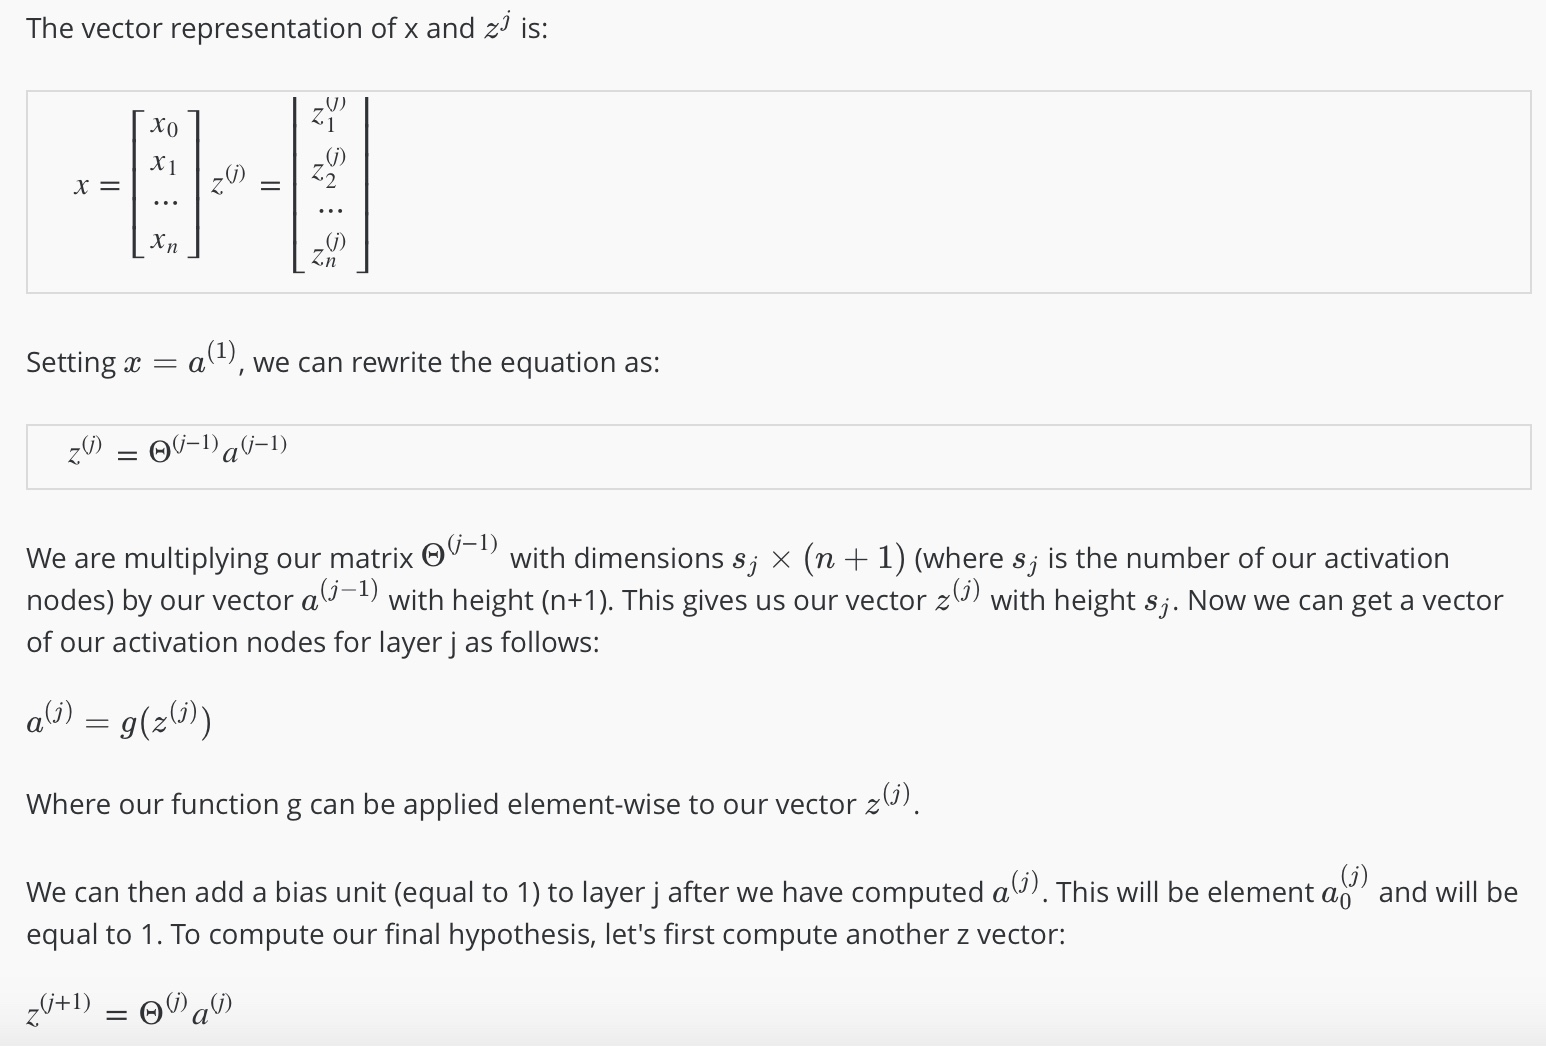
\includegraphics[width=1\textwidth]{./ImagenesW4/modelRep7}
\end{figure}

\begin{figure}[H]
	\centering
	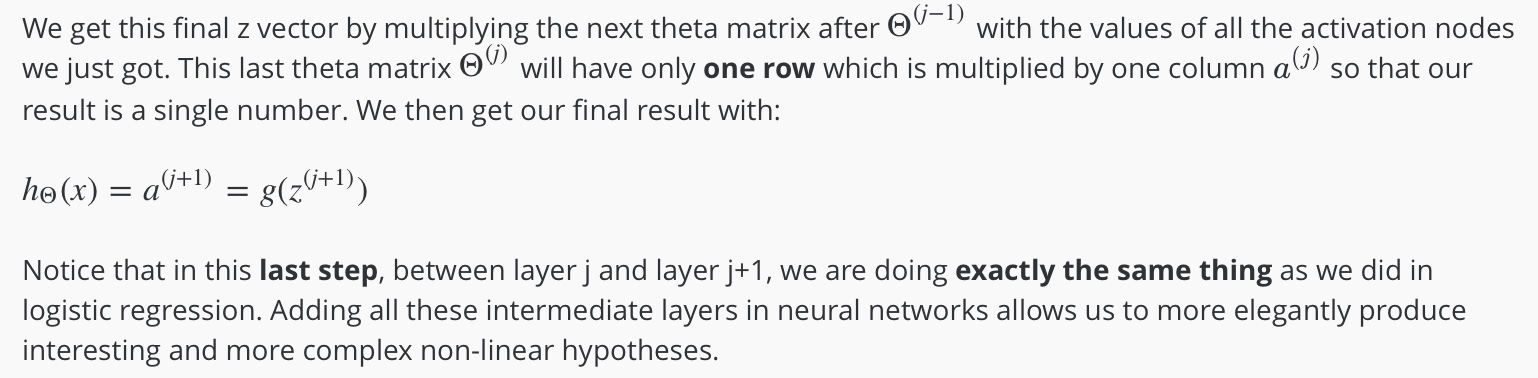
\includegraphics[width=1\textwidth]{./ImagenesW4/modelRep8}
\end{figure}

\begin{figure}[H]
	\centering
	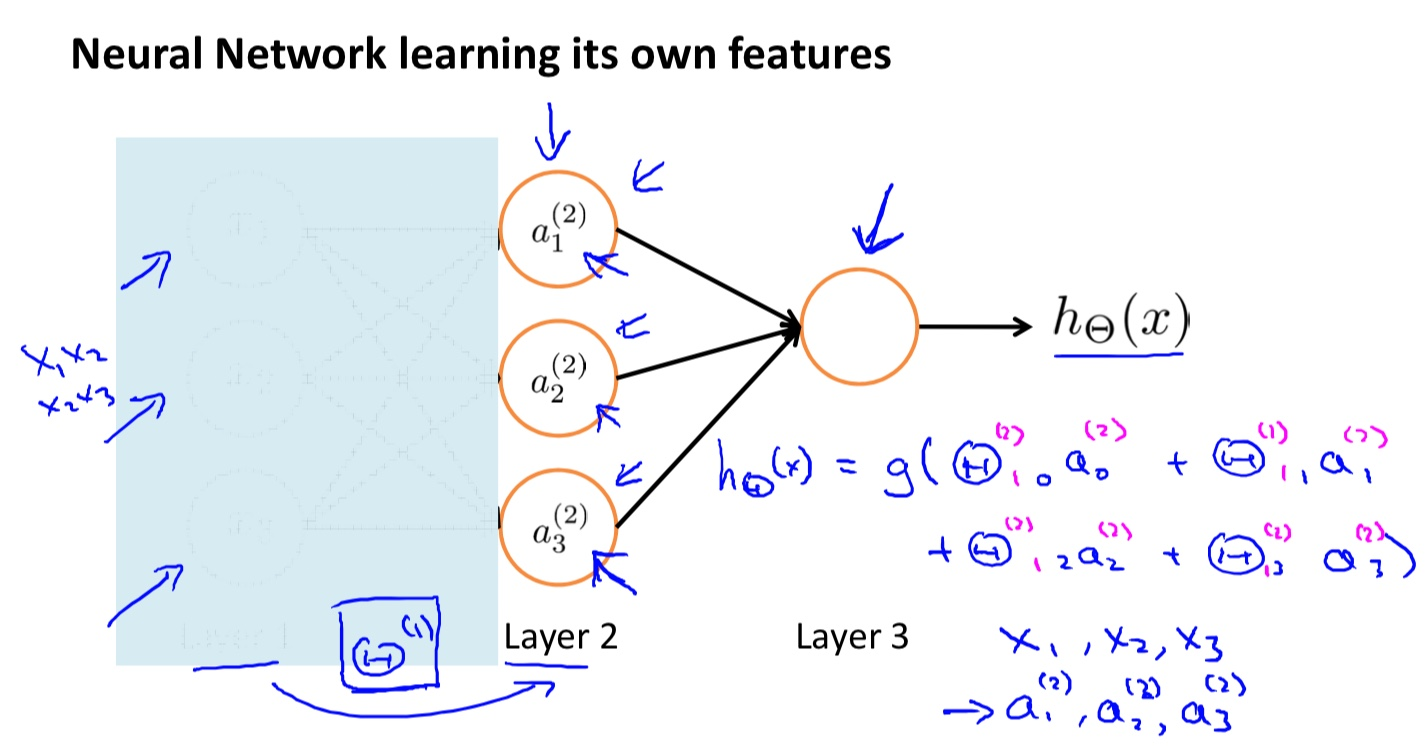
\includegraphics[width=0.8\textwidth]{./ImagenesW4/forwardProp2}
\end{figure}

\begin{figure}[H]
	\centering
	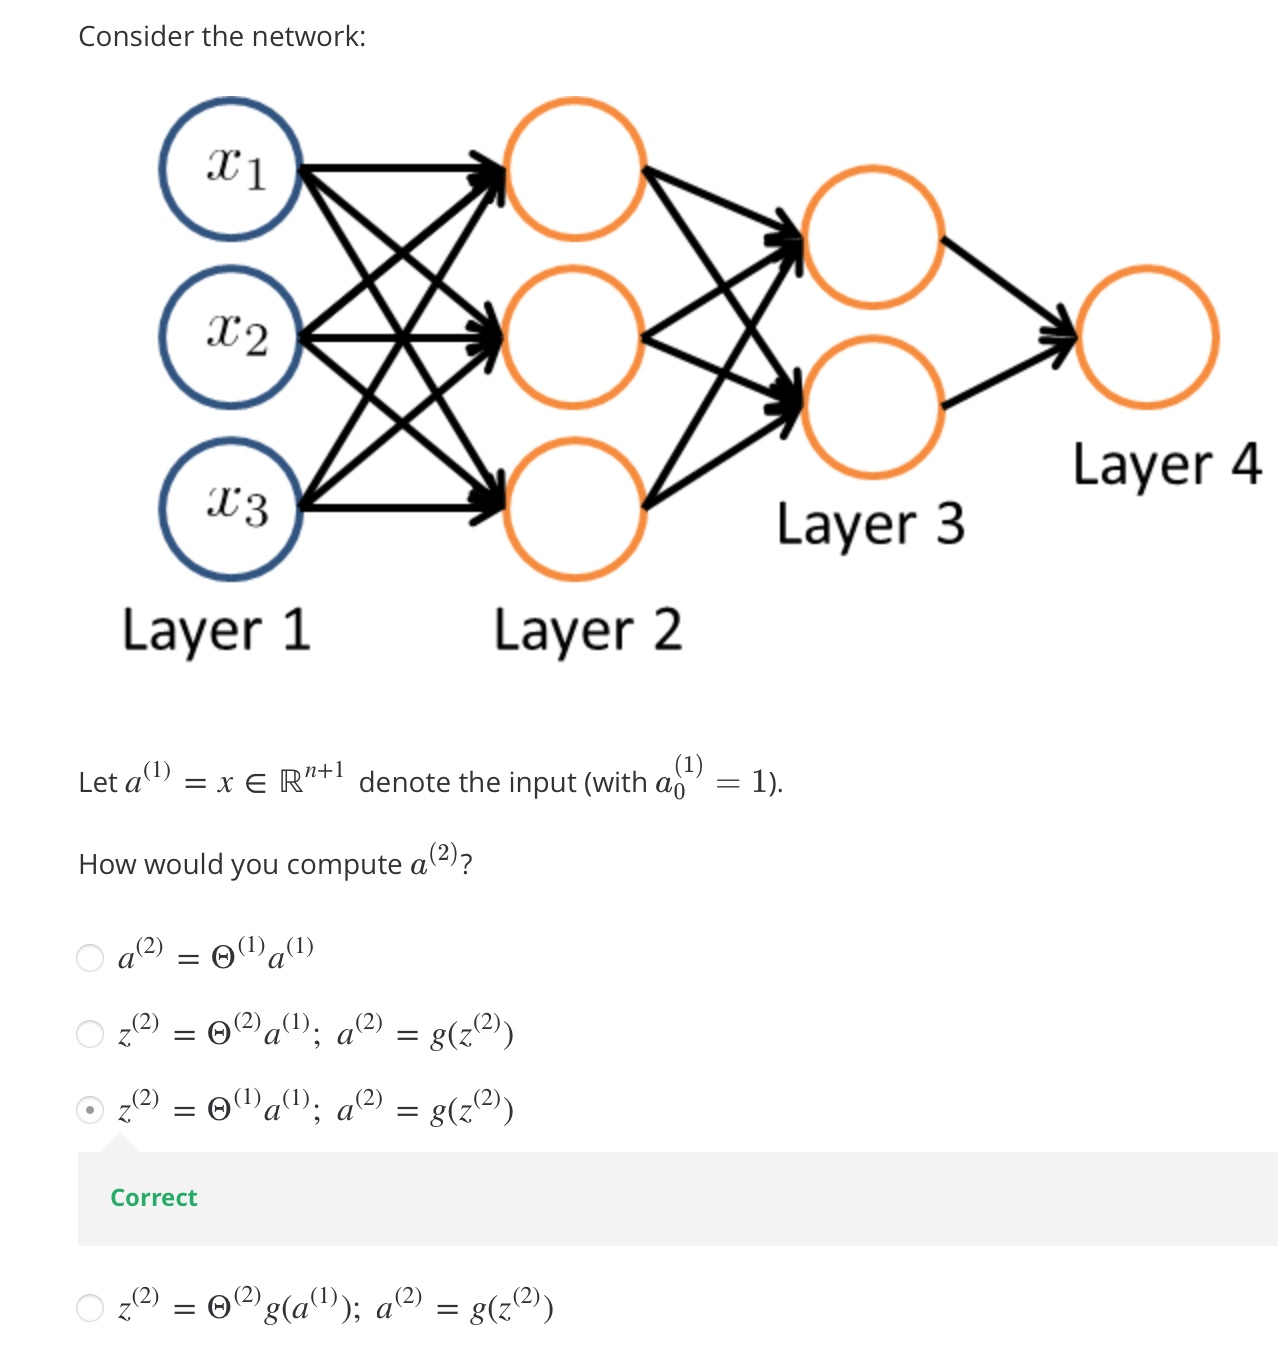
\includegraphics[width=0.8\textwidth]{./ImagenesW4/testmrep2}
\end{figure}



\subsection{Applications}

\subsubsection{Examples}

\begin{figure}[H]
	\centering
	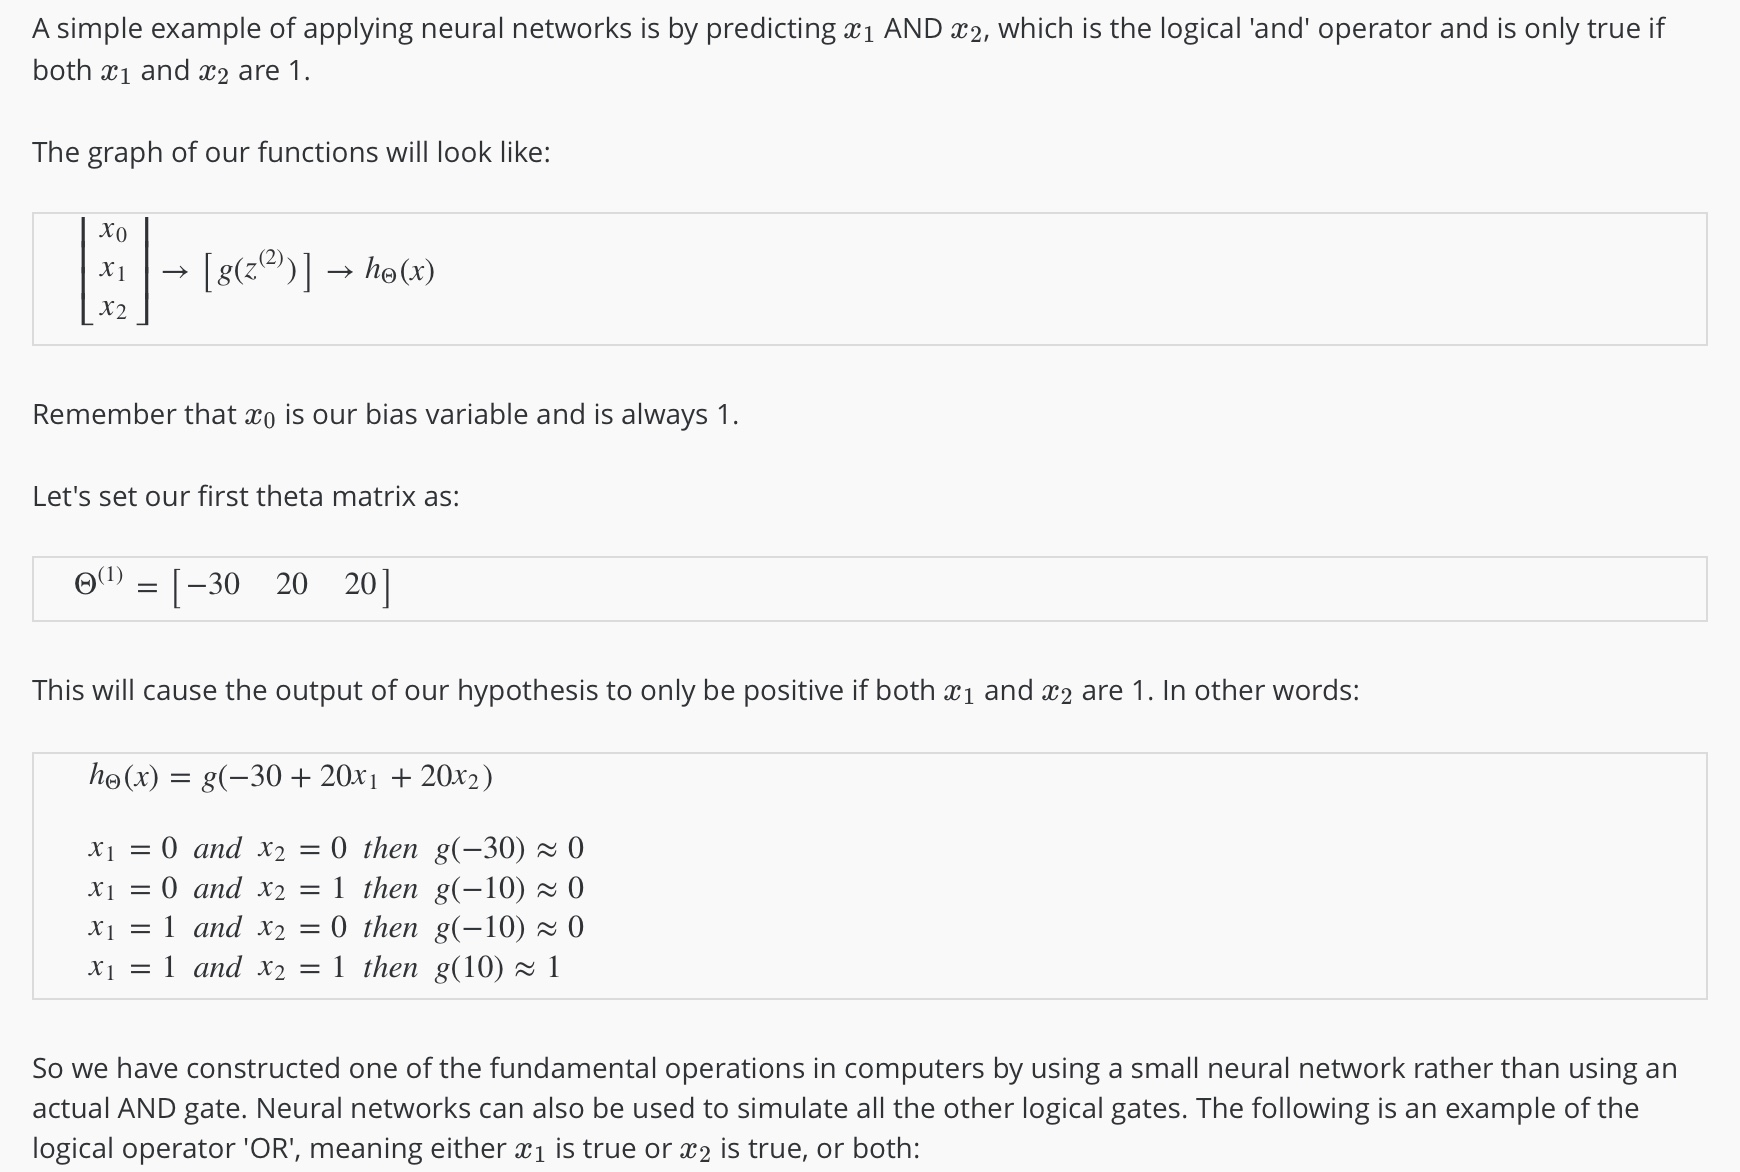
\includegraphics[width=1\textwidth]{./ImagenesW4/examplesI1}
\end{figure}

\begin{figure}[H]
	\centering
	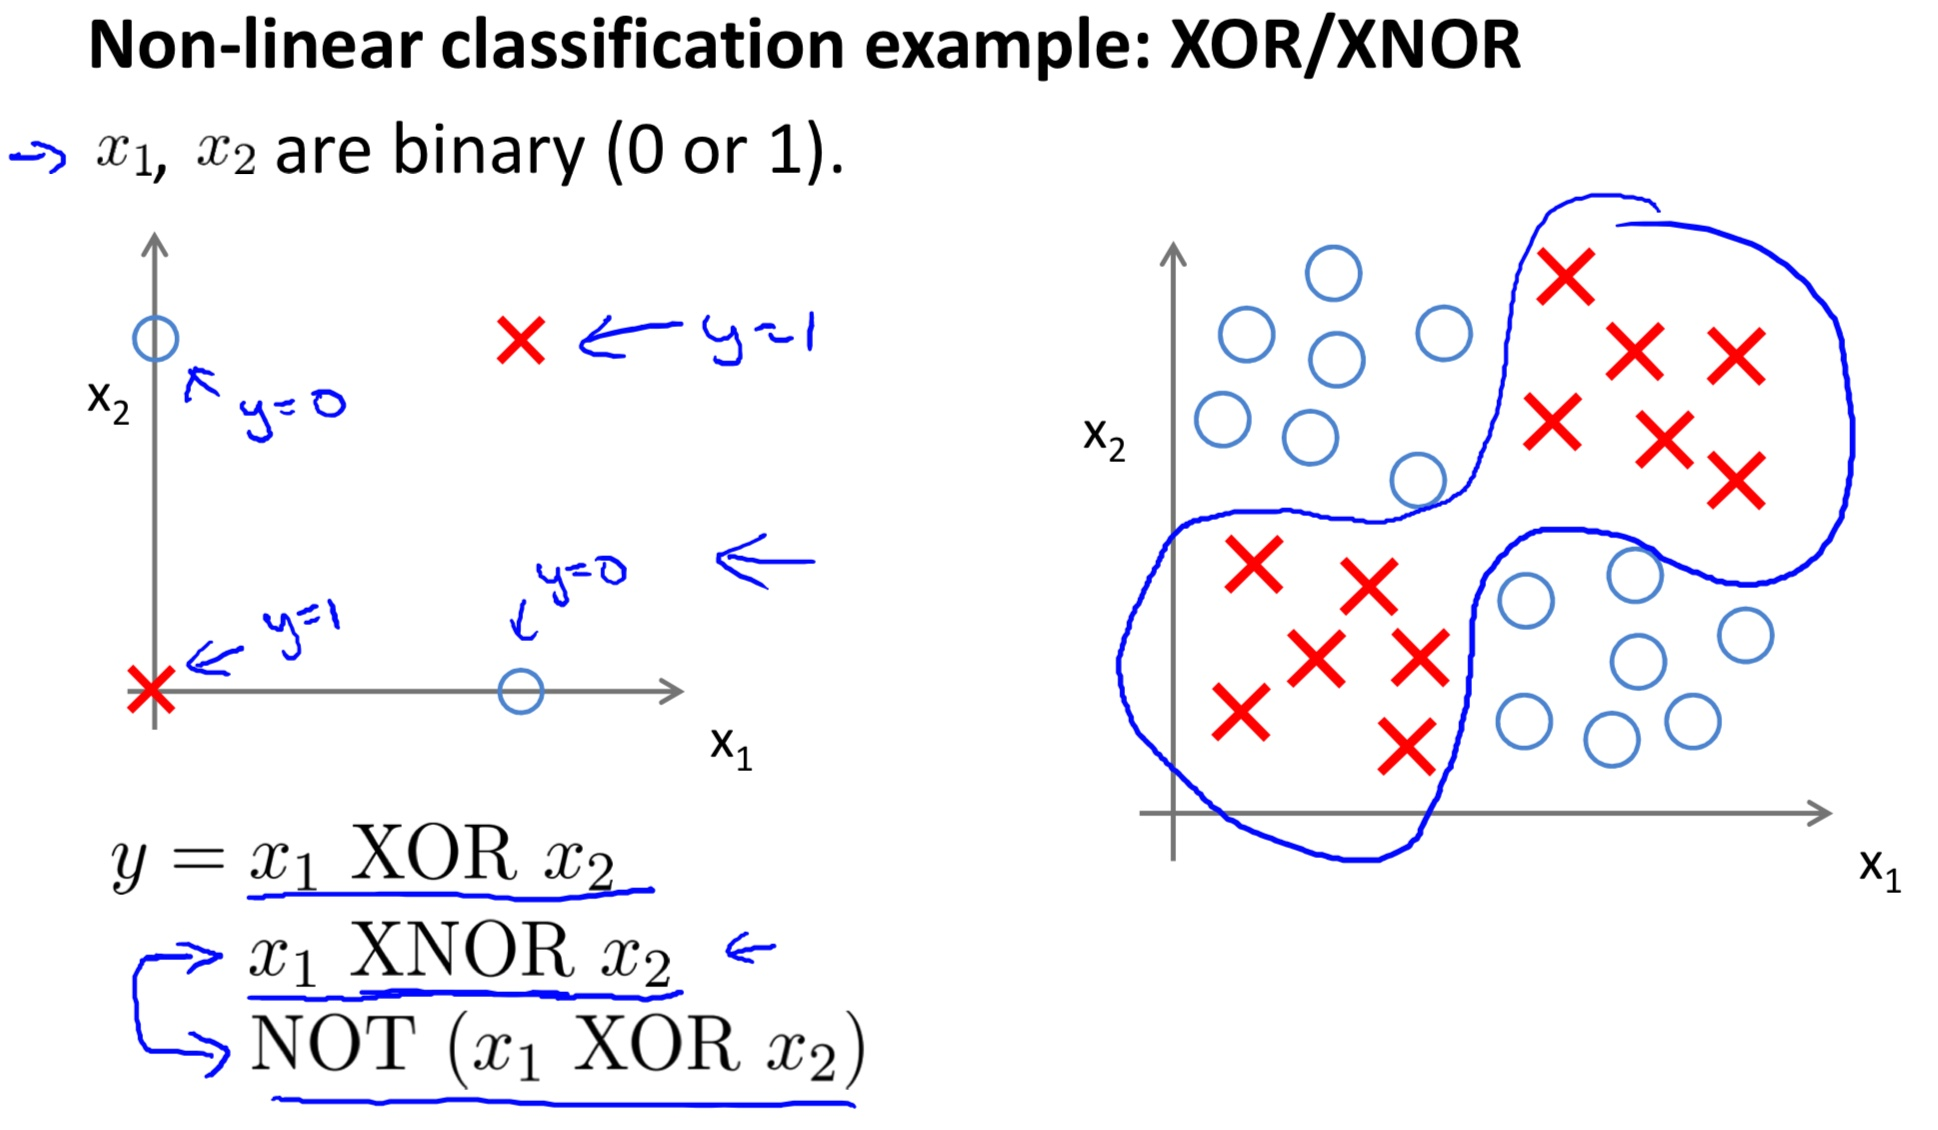
\includegraphics[width=1\textwidth]{./ImagenesW4/xor}
\end{figure}

\begin{figure}[H]
	\centering
	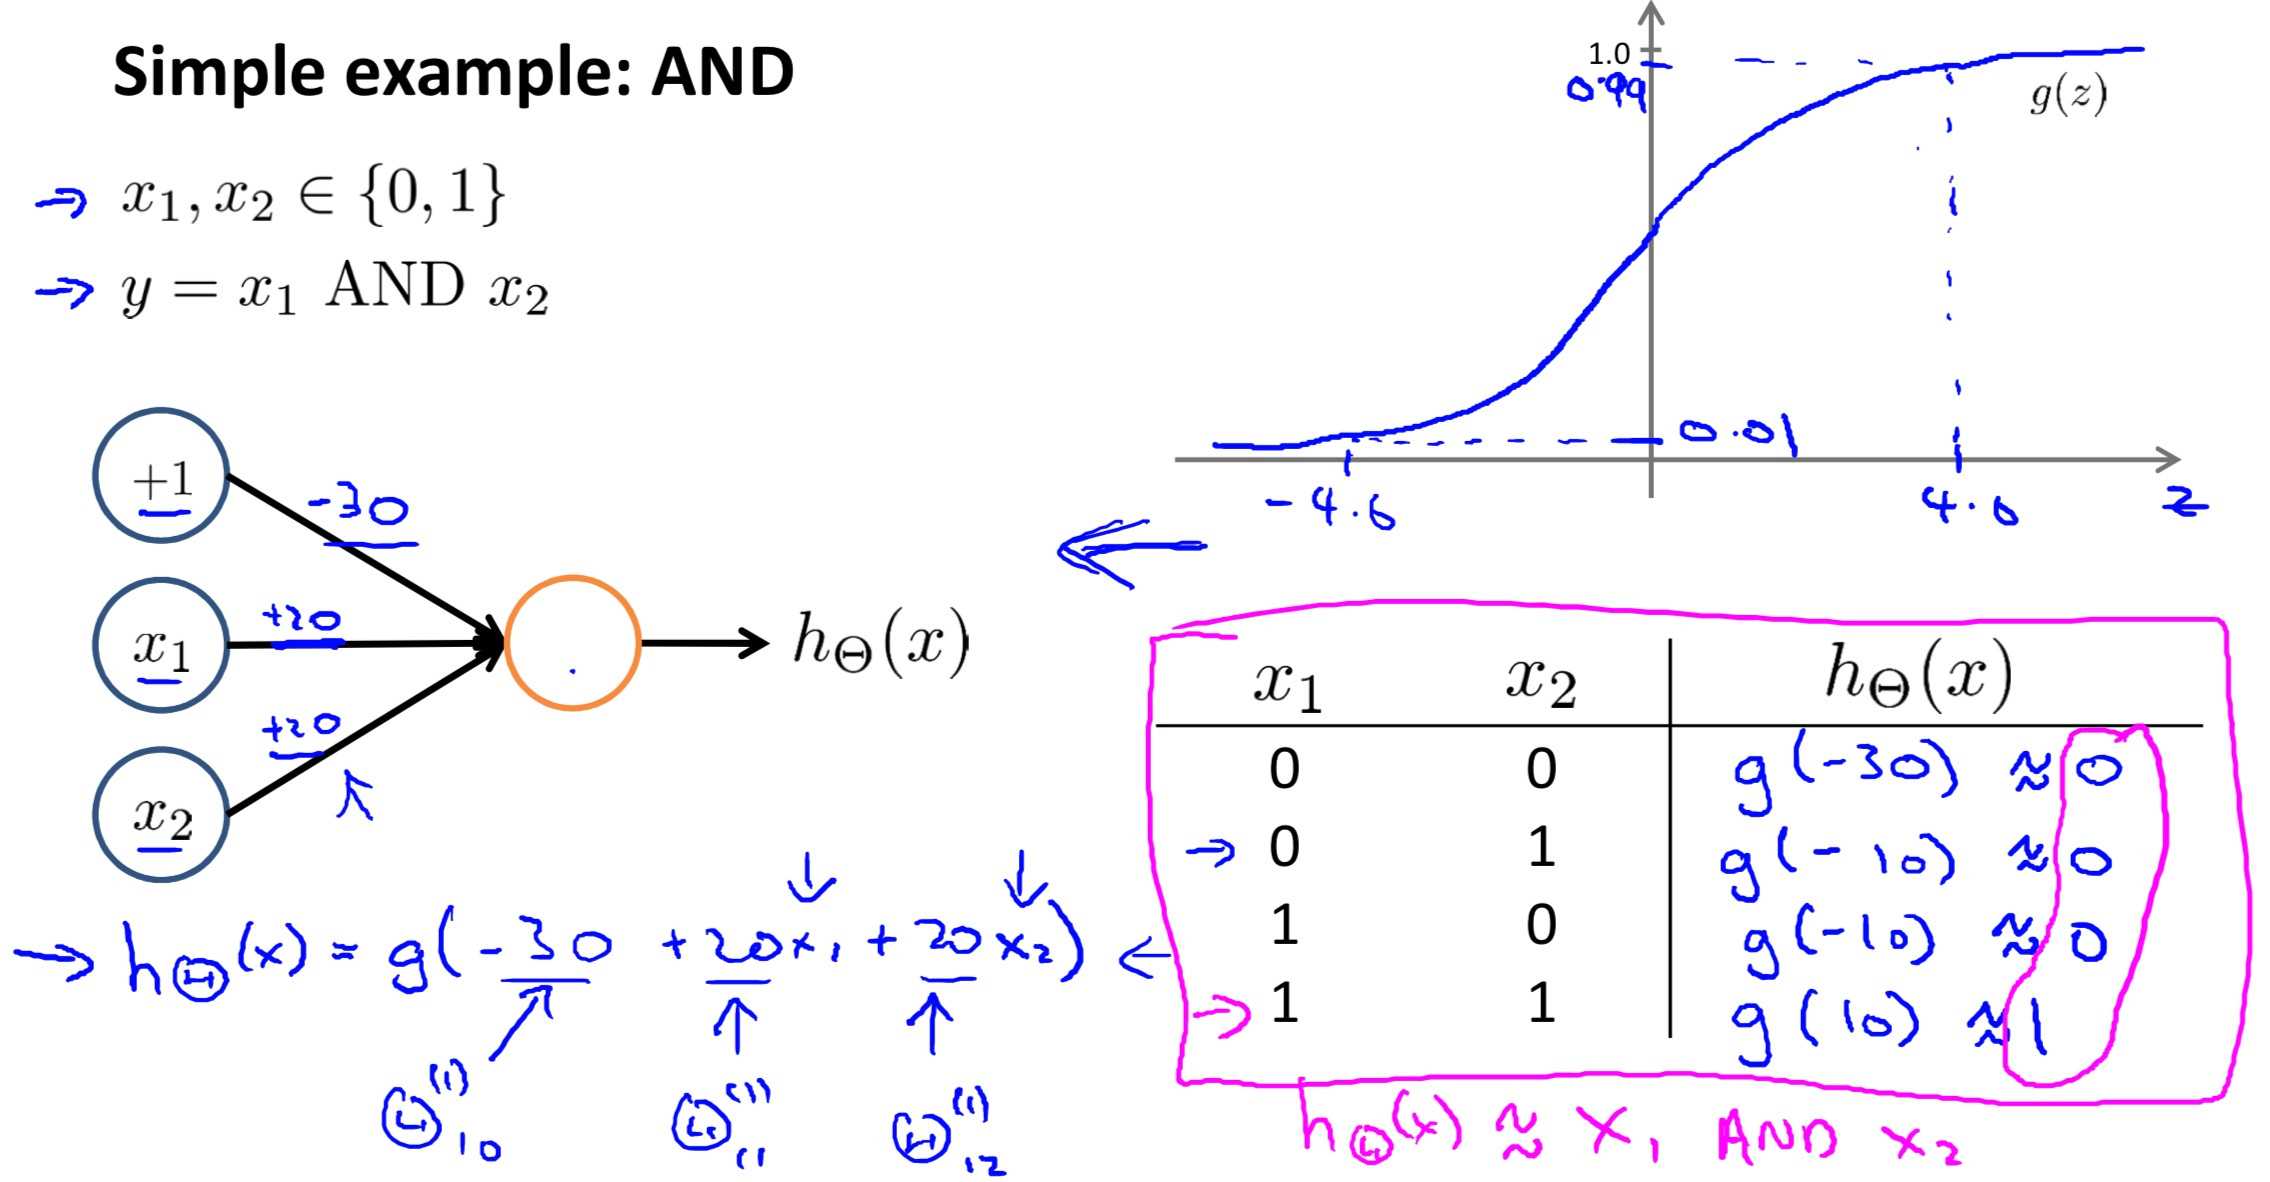
\includegraphics[width=1\textwidth]{./ImagenesW4/and}
\end{figure}

\begin{figure}[H]
	\centering
	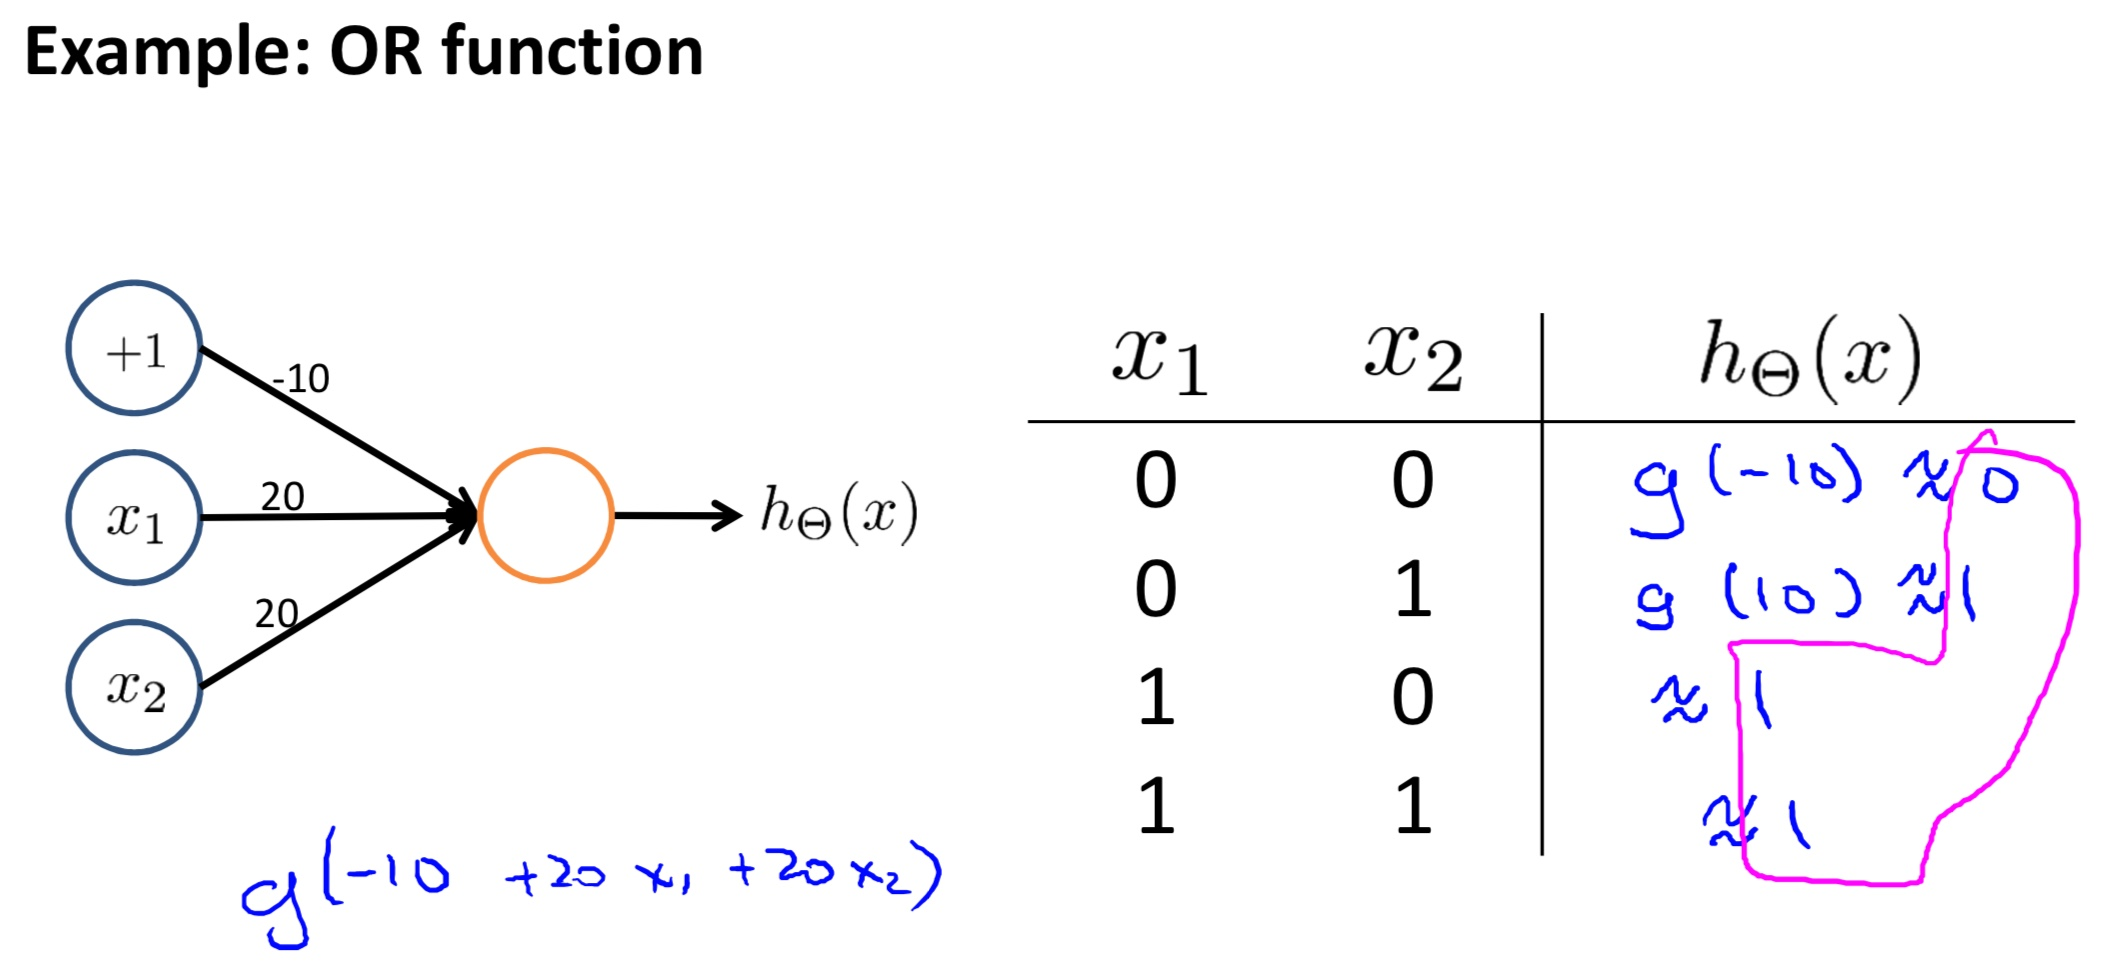
\includegraphics[width=1\textwidth]{./ImagenesW4/or}
\end{figure}

\begin{figure}[H]
	\centering
	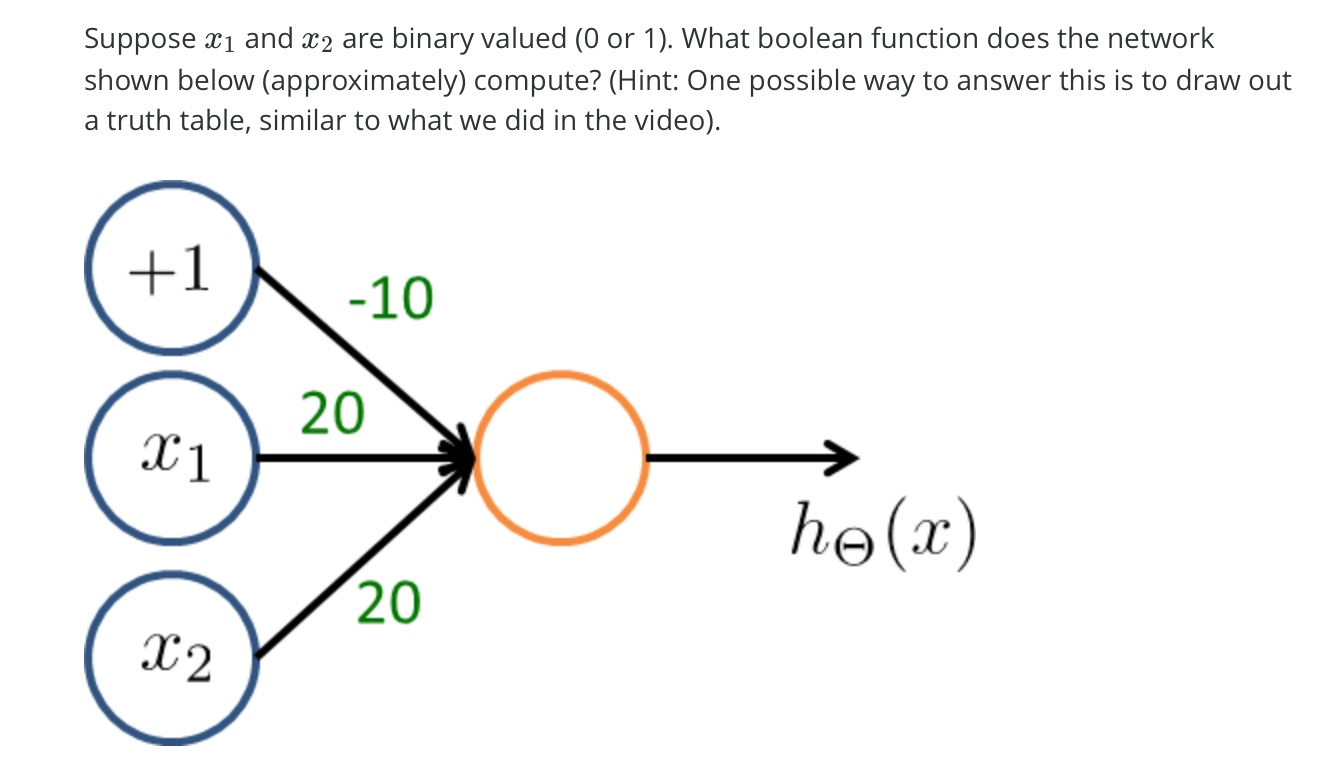
\includegraphics[width=1\textwidth]{./ImagenesW4/testExamplesI_1}
\end{figure}

\begin{figure}[H]
	\centering
	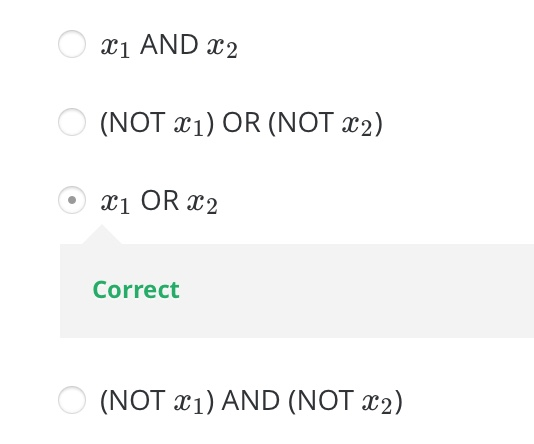
\includegraphics[width=0.7\textwidth]{./ImagenesW4/testExamplesI_2}
\end{figure}


\begin{figure}[H]
	\centering
	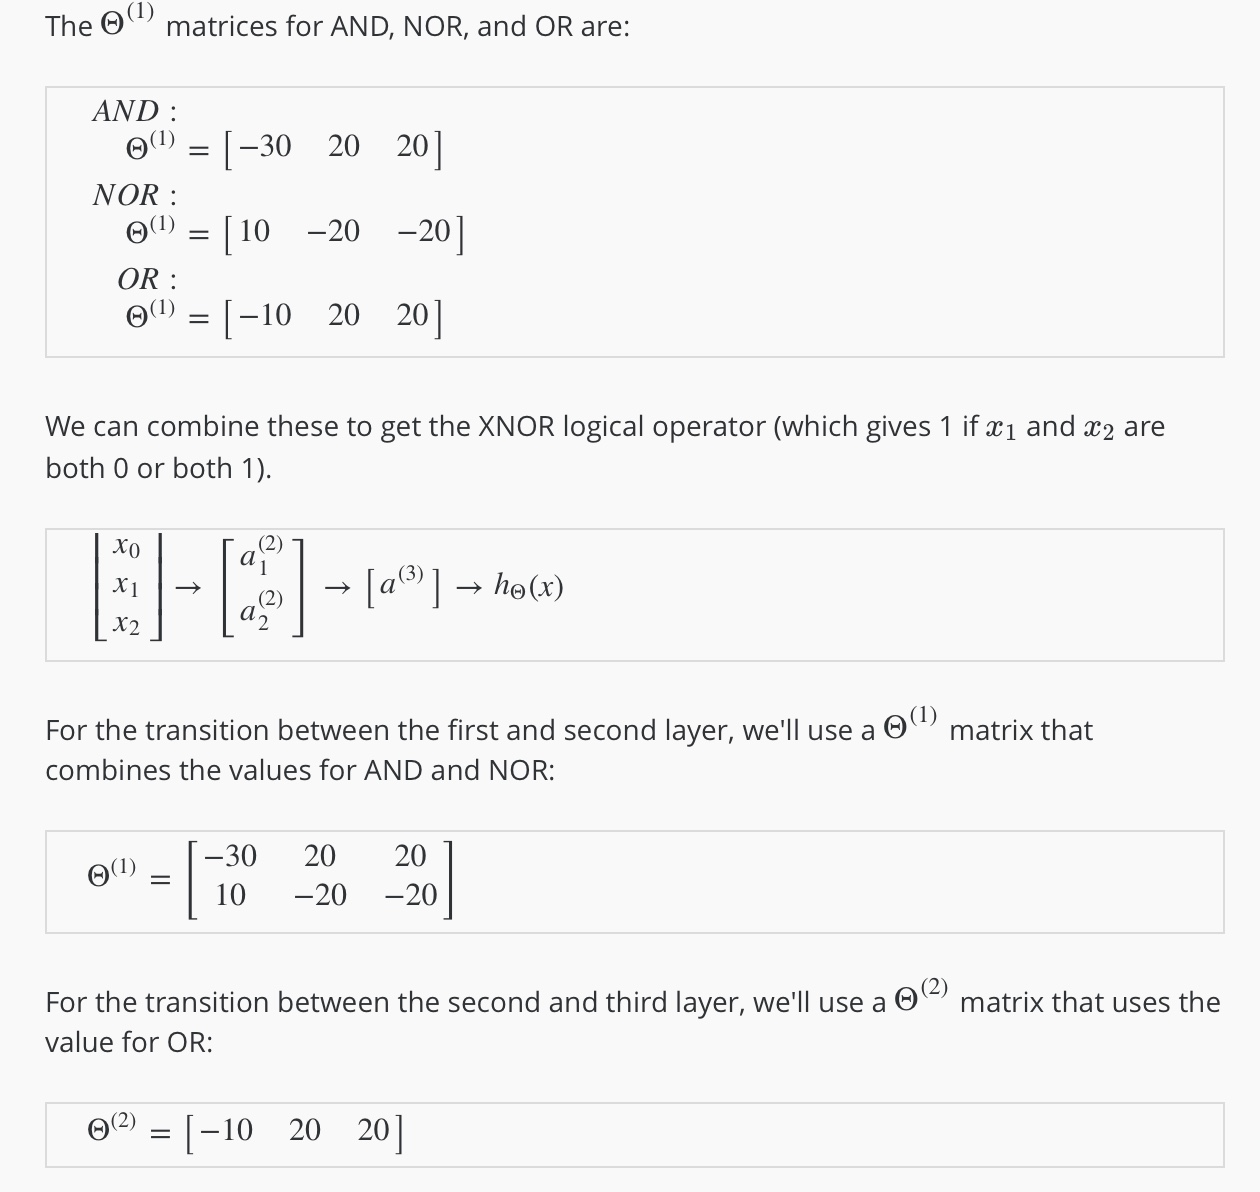
\includegraphics[width=1\textwidth]{./ImagenesW4/examplesII1}
\end{figure}

\begin{figure}[H]
	\centering
	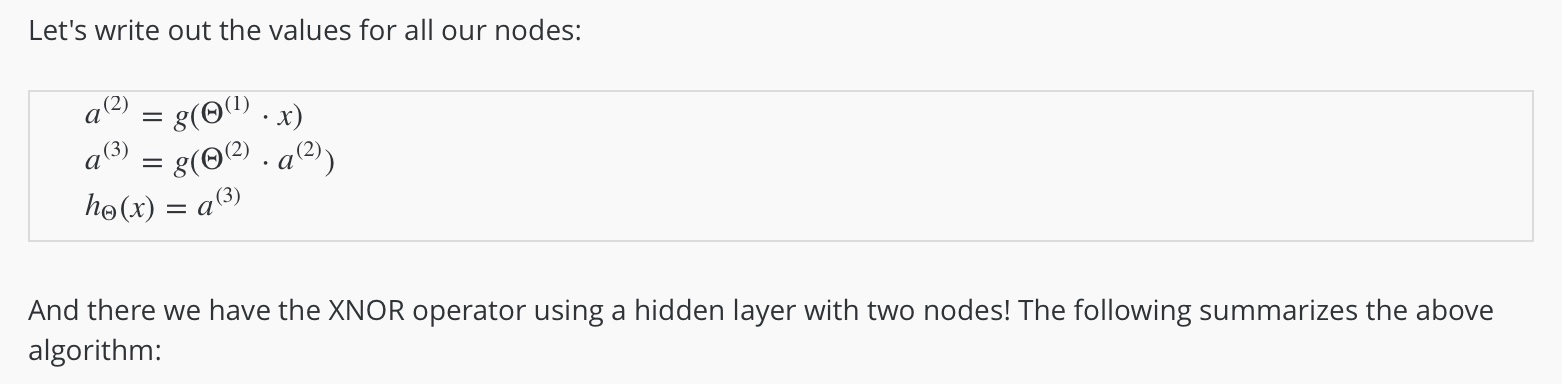
\includegraphics[width=1\textwidth]{./ImagenesW4/examplesII2}
\end{figure}

\begin{figure}[H]
	\centering
	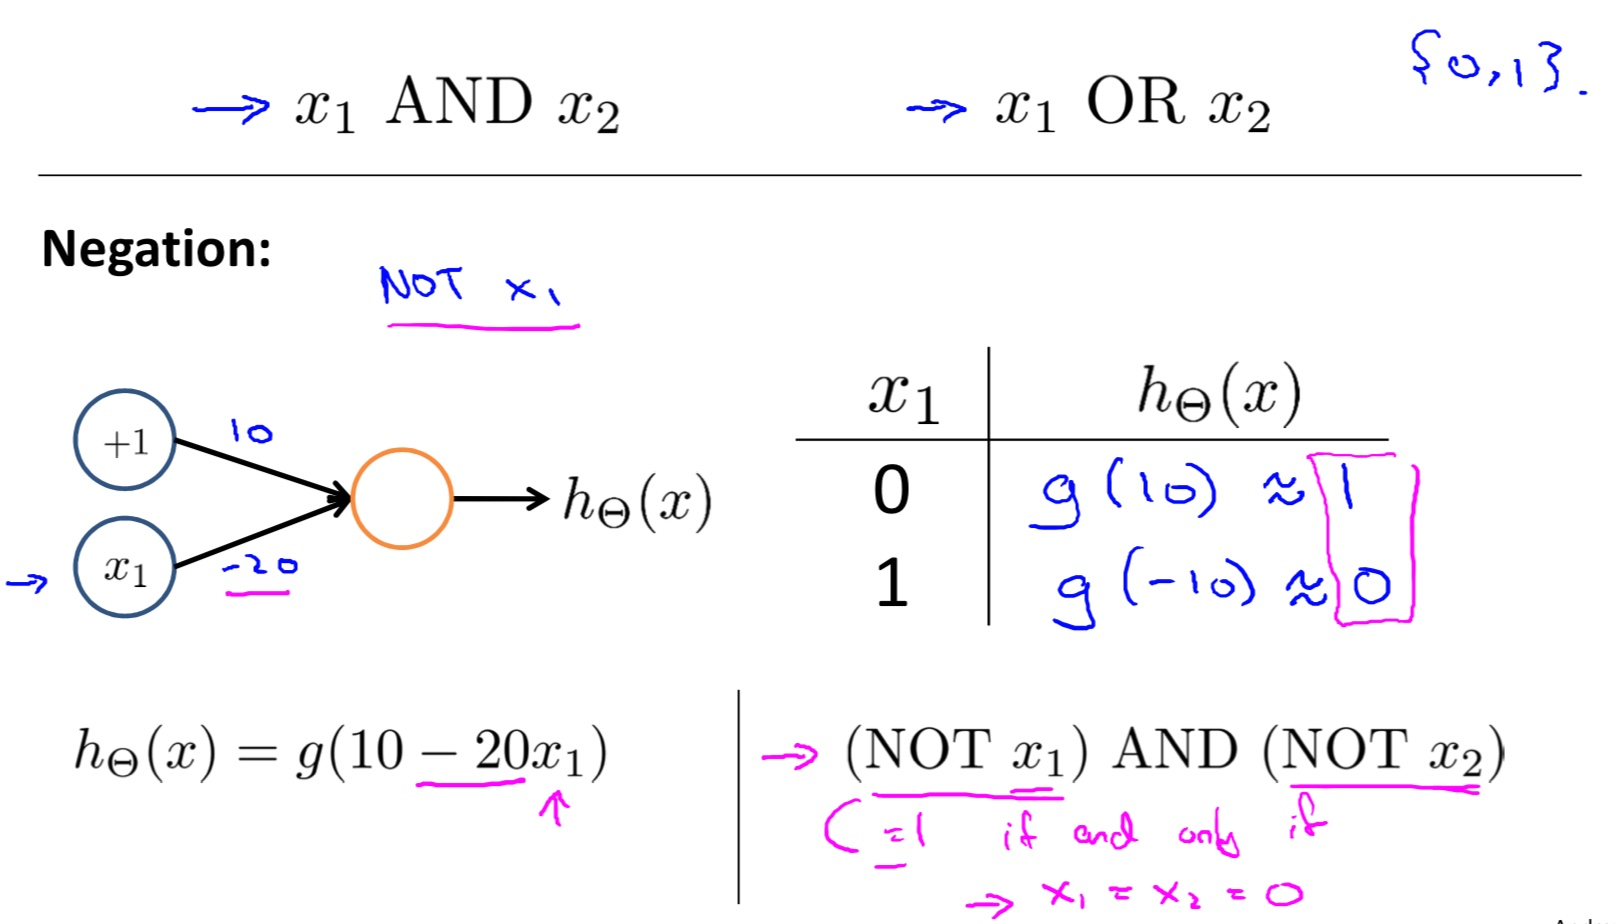
\includegraphics[width=1\textwidth]{./ImagenesW4/andor}
\end{figure}

\begin{figure}[H]
	\centering
	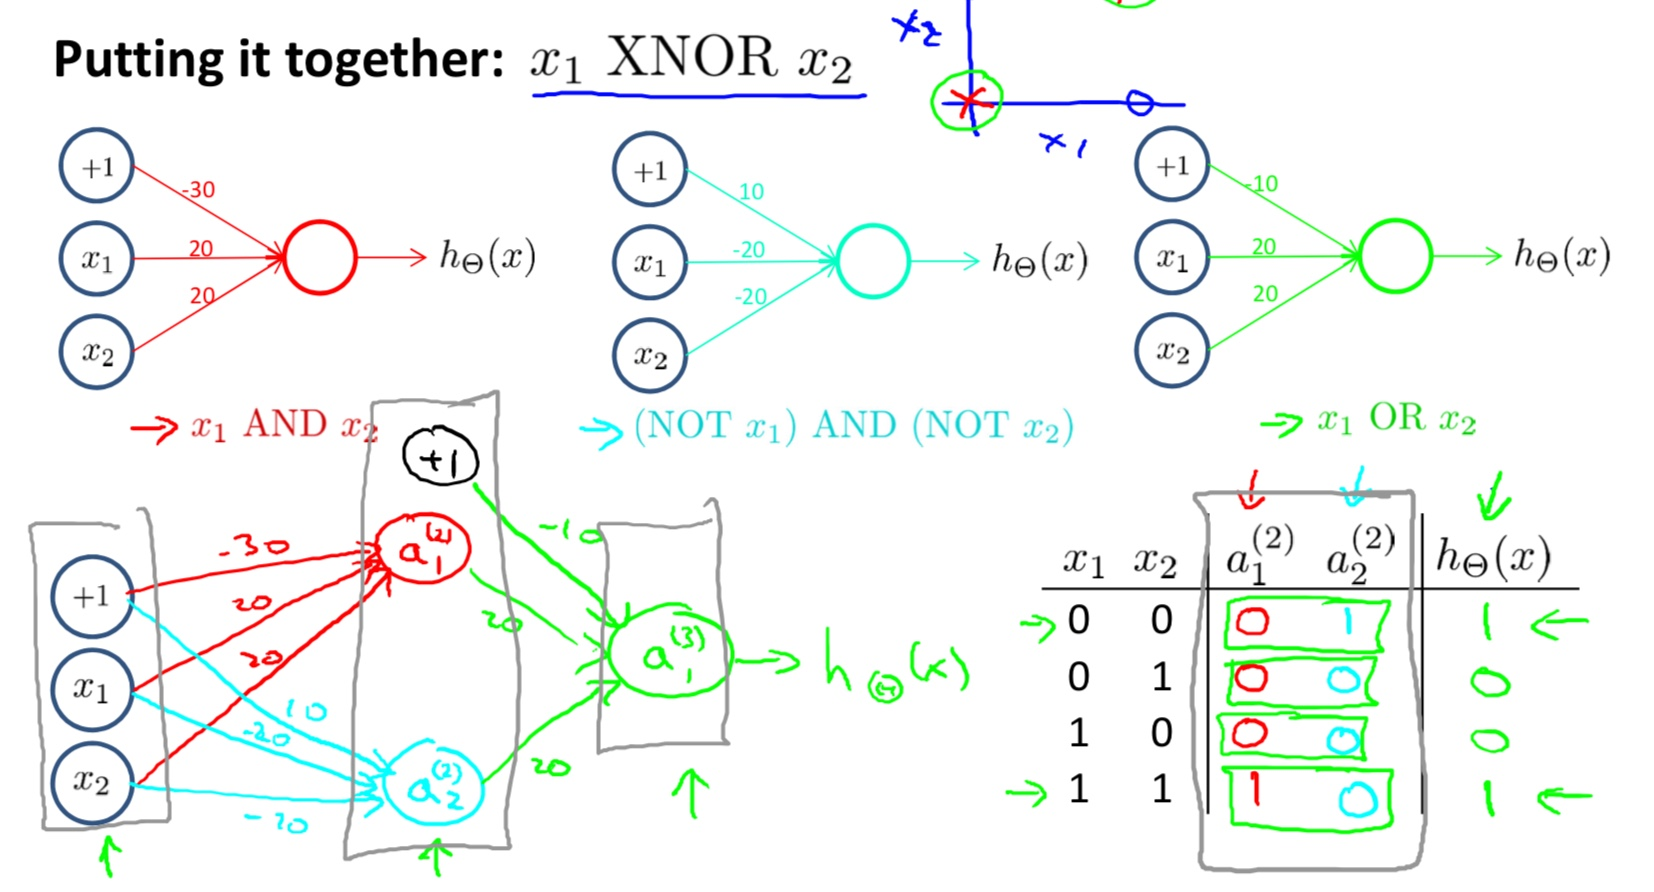
\includegraphics[width=1\textwidth]{./ImagenesW4/xnor}
\end{figure}

\subsubsection{Multiclass classification}

\begin{figure}[H]
	\centering
	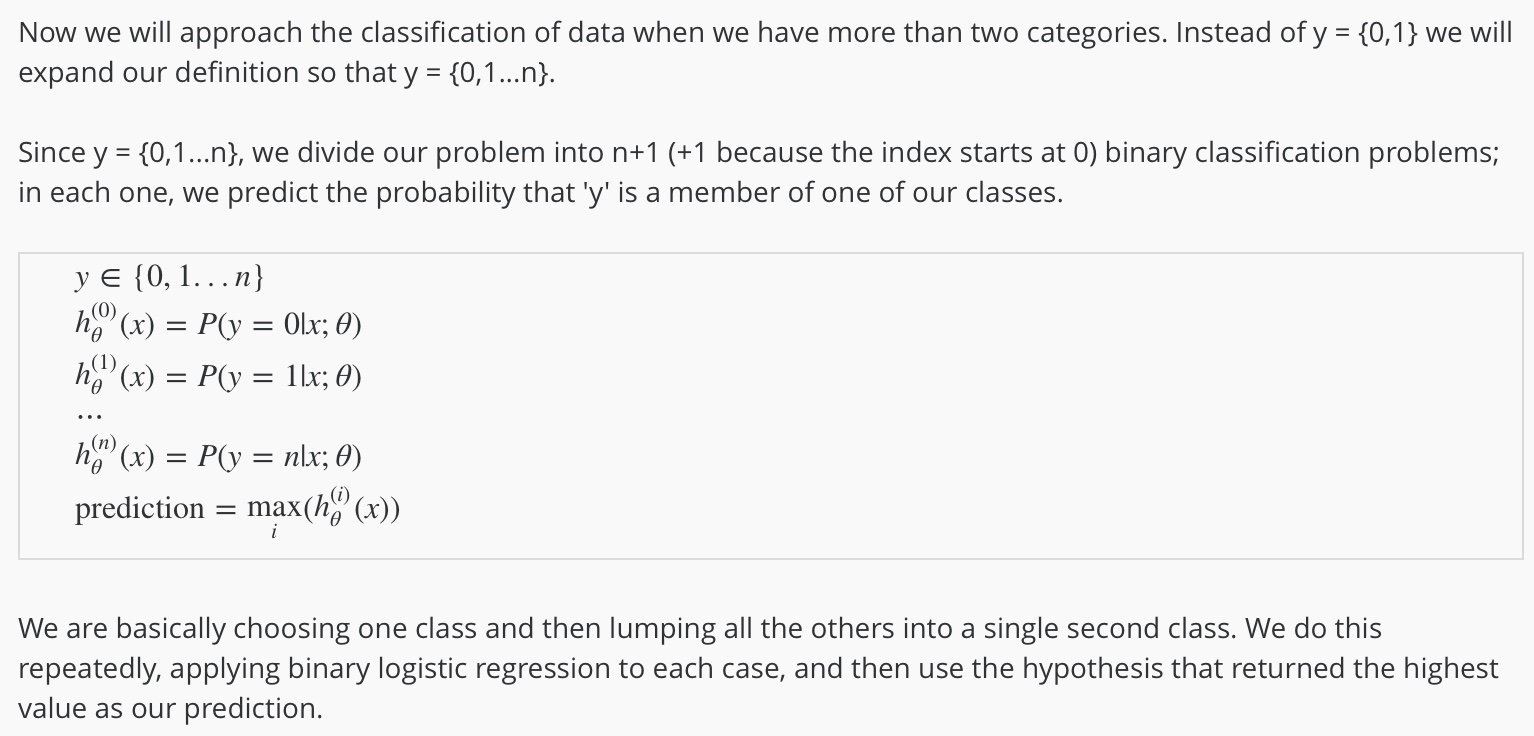
\includegraphics[width=0.85\textwidth]{./ImagenesW4/multiClass1}
\end{figure}

\begin{figure}[H]
	\centering
	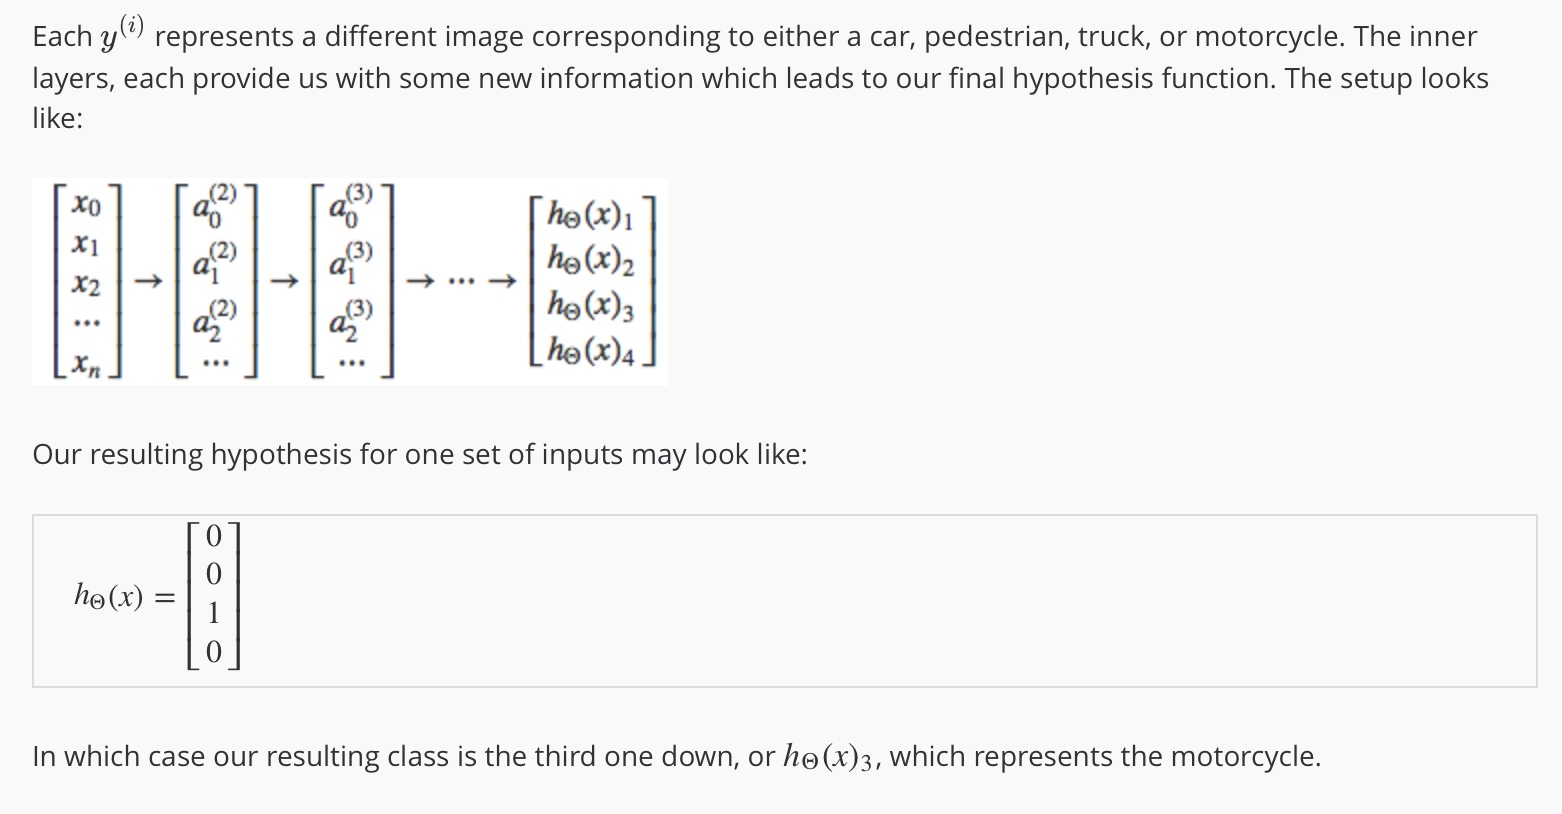
\includegraphics[width=0.85\textwidth]{./ImagenesW4/multiClass2}
\end{figure}

\subsection{Test}

\begin{figure}[H]
	\centering
	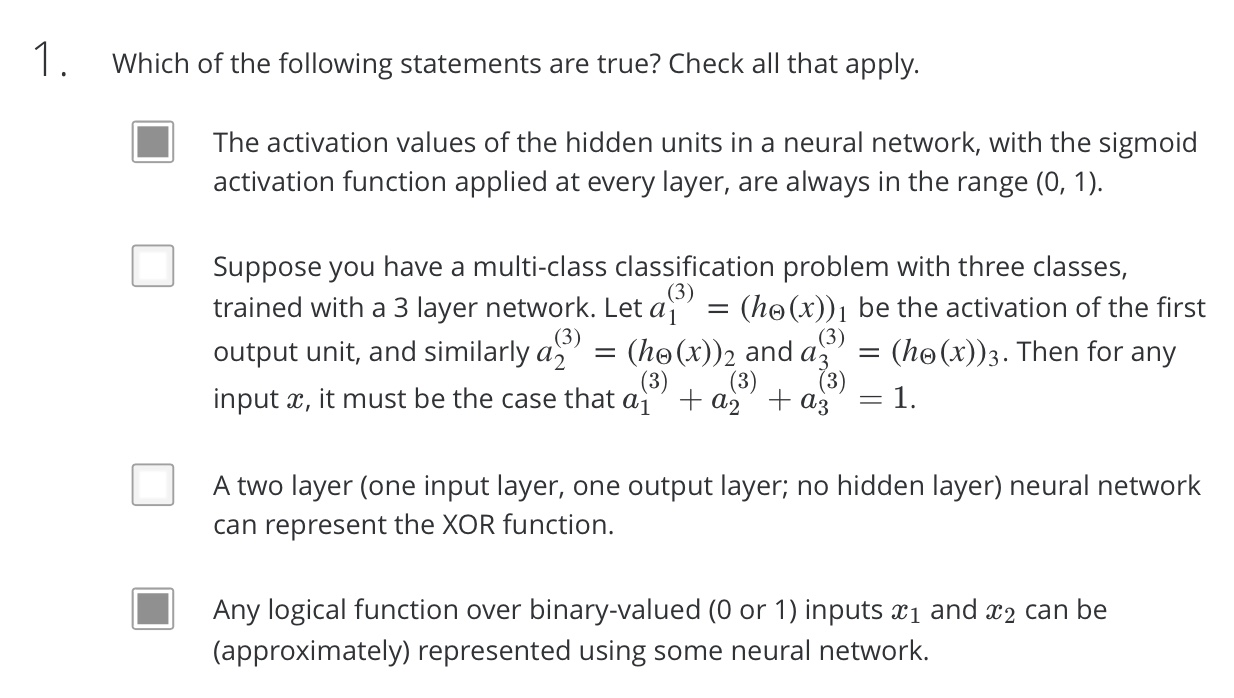
\includegraphics[width=0.85\textwidth]{./ImagenesW4/testNN1}
\end{figure}

\begin{figure}[H]
	\centering
	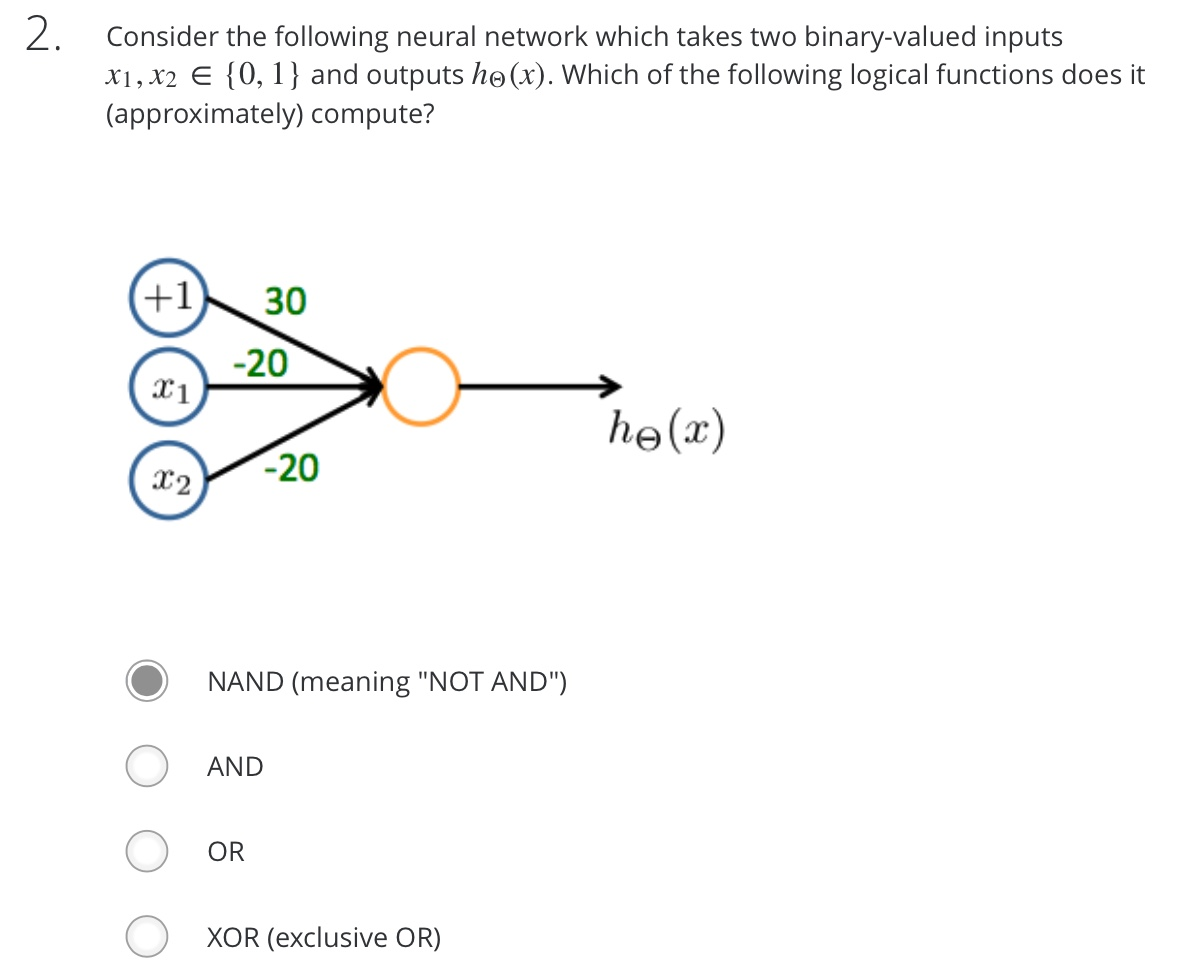
\includegraphics[width=0.85\textwidth]{./ImagenesW4/testNN2}
\end{figure}

\begin{figure}[H]
	\centering
	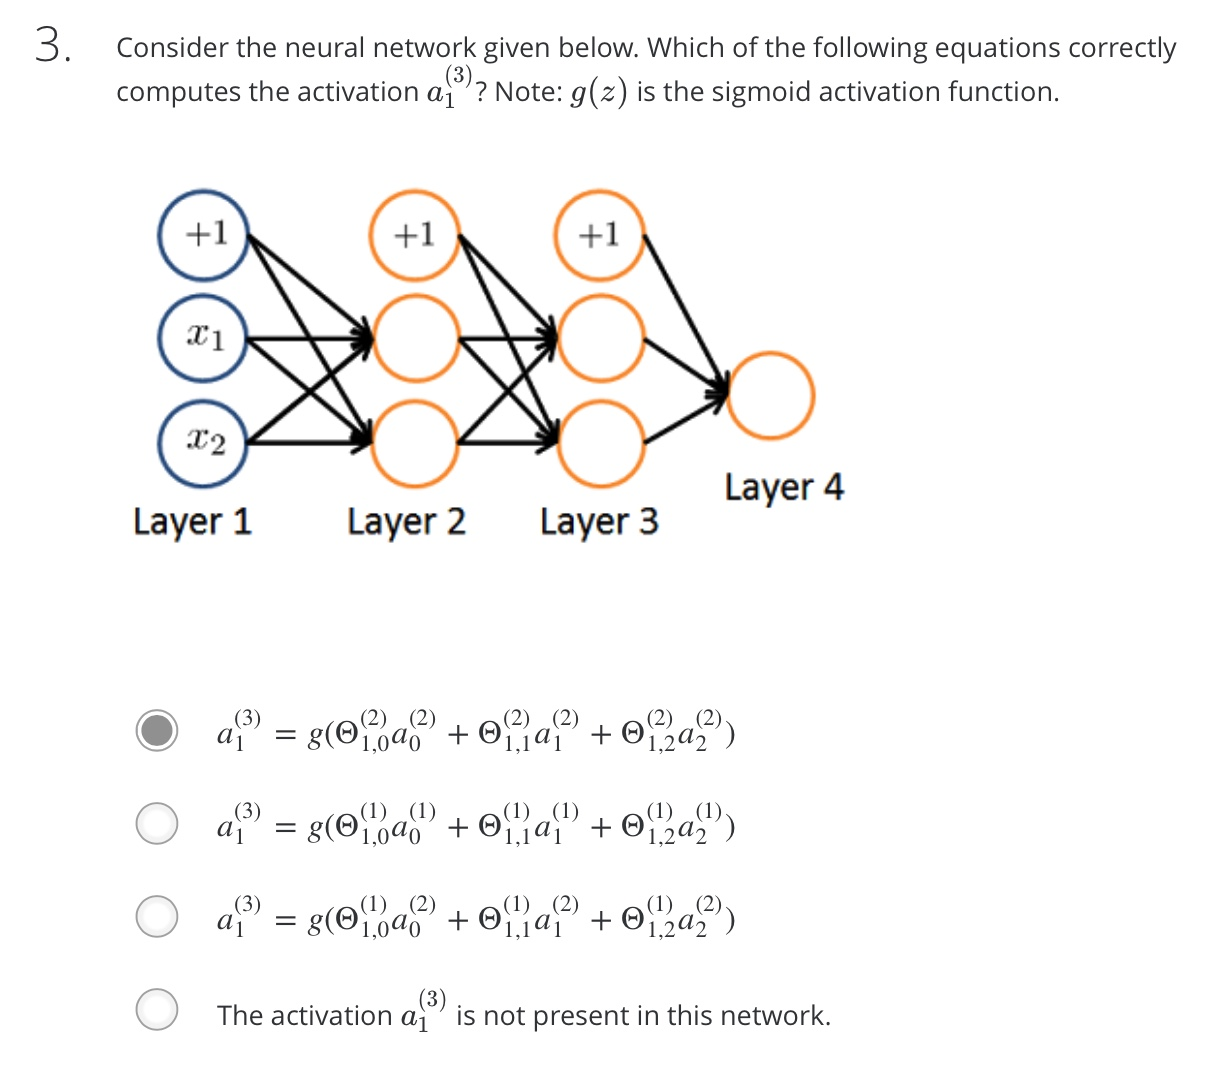
\includegraphics[width=0.8\textwidth]{./ImagenesW4/testNN3}
\end{figure}

\begin{figure}[H]
\minipage{0.5\textwidth}
  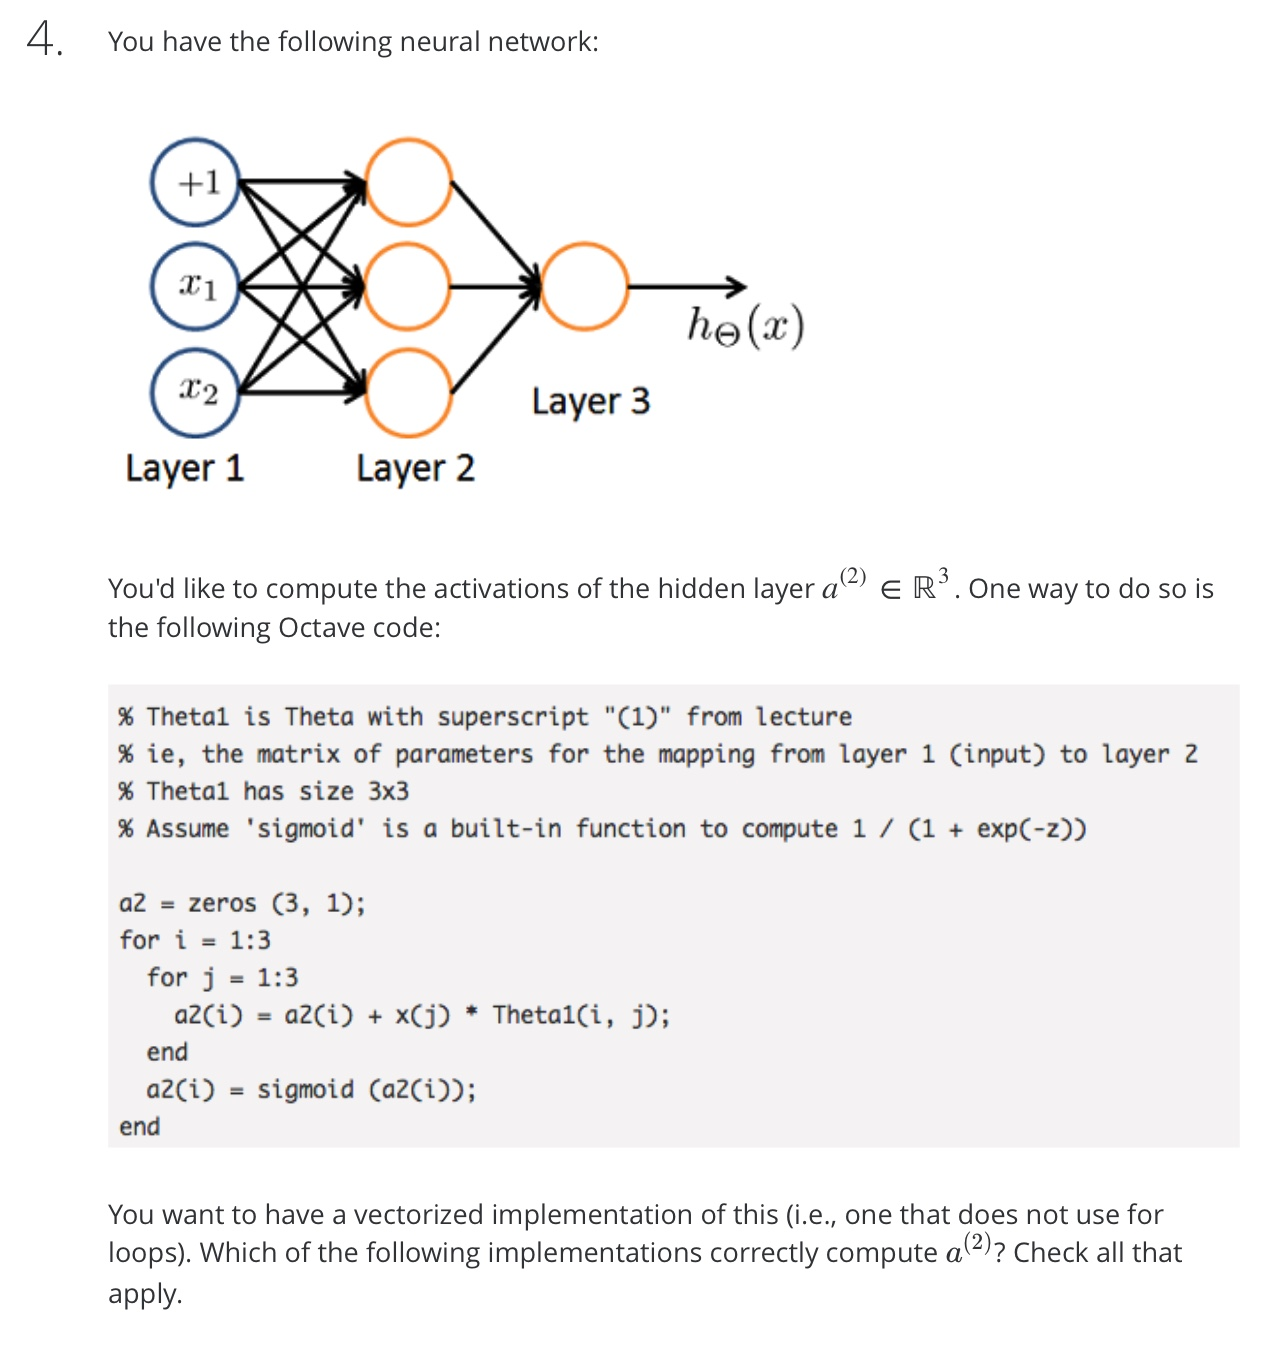
\includegraphics[width=\linewidth]{./ImagenesW4/testNN4_1}
\endminipage\hfill
\minipage{0.525\textwidth}
  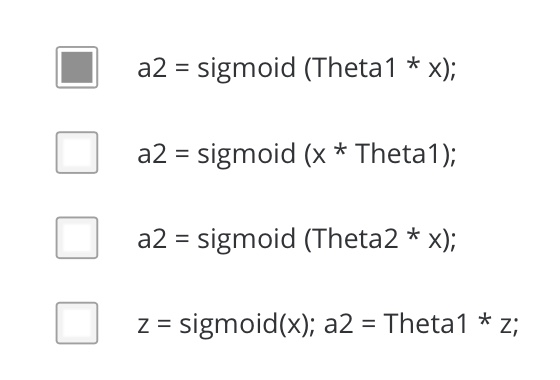
\includegraphics[width=\linewidth]{./ImagenesW4/testNN4_2}
\endminipage\hfill
\end{figure}

\begin{figure}[H]
	\centering
	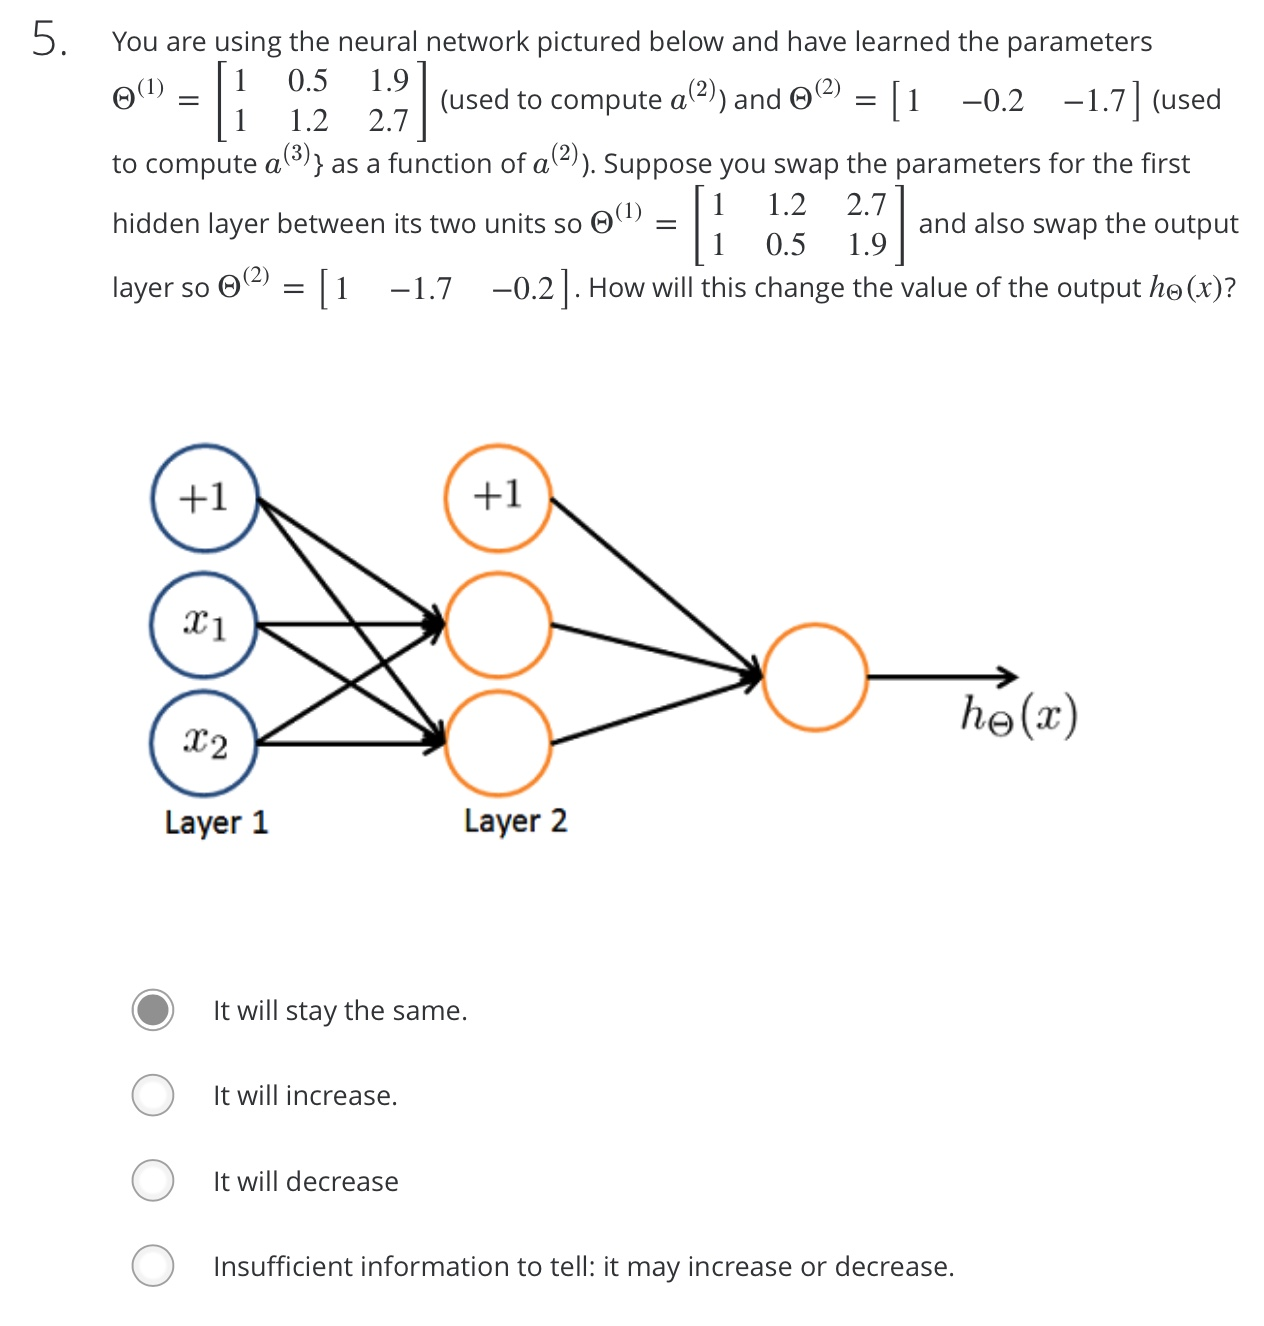
\includegraphics[width=0.85\textwidth]{./ImagenesW4/testNN5}
\end{figure}

%\begin{figure}[H]
%	\centering
%	\includegraphics[width=1\textwidth]{./Imagenes/prueba}
%\end{figure}


\end{document}
